%%
%% This is file `sample-nime-paper.tex',
%% generated with the docstrip utility.
%%
%% The original source files were:
%%
%% samples.dtx  (with options: `all,proceedings,bibtex,sigconf')
%% 
%% IMPORTANT NOTICE:
%% 
%% For the copyright see the source file.
%% 
%% Any modified versions of this file must be renamed
%% with new filenames distinct from sample-nime-paper.tex.
%% 
%% For distribution of the original source see the terms
%% for copying and modification in the file samples.dtx.
%% 
%% This generated file may be distributed as long as the
%% original source files, as listed above, are part of the
%% same distribution. (The sources need not necessarily be
%% in the same archive or directory.)
%%
%%
%% Commands for TeXCount
%TC:macro \cite [option:text,text]
%TC:macro \citep [option:text,text]
%TC:macro \citet [option:text,text]
%TC:envir table 0 1
%TC:envir table* 0 1
%TC:envir tabular [ignore] word
%TC:envir displaymath 0 word
%TC:envir math 0 word
%TC:envir comment 0 0
%%
%%
%% History of NIME Template Updaters:
%% Modified by Florent Berthaut, Charles Martin, Yichen Wang, 21 November 2024
%% Modified by Adnan Marquez-Borbon 30 November 2022
%% Modified by Courtney Reed 28 November 2022
%% Modified by Joe Wright 14 December 2019
%% Modified by Niccolò Granieri 10 October 2018
%% Modified by Angelo Fraietta 23 December 2018
%% Modified by Angelo Fraietta 22 November 2018
%% Modified by Rodrigo Schramm on 22 September 2018
%% Modified by Luke Dahl on 17 October 2-17
%% Modified by Cumhur Erkut on <2016-10-11 Tue>
%% Modified by Edgar Berdahl on 5 November 2014
%% Modified by Baptiste Caramiaux on 25 November 2013
%% Modified by Kyogu Lee on 7 October 2012
%% Modified by Georg Essl on 7 November 2011
%%
%% And here's the template:
%%
%% The first command in your LaTeX source must be the \documentclass
%% command.
%%
%% For submission and review of your manuscript please change the
%% command to \documentclass[manuscript, screen, review]{nimeart}.
%%
%% When submitting camera ready or to TAPS, please change the command
%% to \documentclass[sigconf]{nimeart} or whichever template is required
%% for your publication.
%%
%%
\documentclass[sigconf]{nimeart}
\usepackage{graphicx}
\usepackage{tikz}
\usetikzlibrary{shapes,arrows}

%%
%% \BibTeX command to typeset BibTeX logo in the docs
\AtBeginDocument{%
  \providecommand\BibTeX{{%
    Bib\TeX}}}

%% Rights management information.  This information is sent to you
%% when you complete the rights form.  These commands have SAMPLE
%% values in them; it is your responsibility as an author to replace
%% the commands and values with those provided to you when you
%% complete the rights form.
\setcopyright{cc}
\copyrightyear{2025}
\acmYear{2025}
\acmDOI{}
%% These commands are for a PROCEEDINGS abstract or paper.
%% Make sure this is up to date with the correct edition of NIME.
\acmConference[NIME '25]{International Conference on New Interfaces for Musical Expression}{June 24--27,
  2025}{Canberra, Australia}
%% This suppresses the ACM Reference Format printing.
\settopmatter{printacmref=false}
%%
%%  Uncomment \acmBooktitle if the title of the proceedings is different
%%  from ``Proceedings of ...''!
%%
%%\acmBooktitle{Woodstock '18: ACM Symposium on Neural Gaze Detection,
%%  June 03--05, 2018, Woodstock, NY}
\acmISBN{}


%%
%% Submission ID.
%% Use this when submitting an article to a sponsored event. You'll
%% receive a unique submission ID from the organizers
%% of the event, and this ID should be used as the parameter to this command.
%%\acmSubmissionID{123-A56-BU3}

%%
%% For managing citations, it is recommended to use bibliography
%% files in BibTeX format.
%%
%% You can then either use BibTeX with the ACM-Reference-Format style,
%% or BibLaTeX with the acmnumeric or acmauthoryear sytles, that include
%% support for advanced citation of software artefact from the
%% biblatex-software package, also separately available on CTAN.
%%
%% Look at the sample-*-biblatex.tex files for templates showcasing
%% the biblatex styles.
%%

%%
%% The majority of ACM publications use numbered citations and
%% references.  The command \citestyle{authoryear} switches to the
%% "author year" style.
%%
%% If you are preparing content for an event
%% sponsored by ACM SIGGRAPH, you must use the "author year" style of
%% citations and references.
%% Uncommenting
%% the next command will enable that style.
%%\citestyle{acmauthoryear}


%%
%% end of the preamble, start of the body of the document source.
\begin{document}

%%
%% The "title" command has an optional parameter,
%% allowing the author to define a "short title" to be used in page headers.
\title{Augmentation of a Historical Harpsichord Keyboard Replica for Haptic-Enabled Interaction in Museum Exhibitions}

%%
%% The "author" command and its associated commands are used to define
%% the authors and their affiliations.
%% Of note is the shared affiliation of the first two authors, and the
%% "authornote" and "authornotemark" commands
%% used to denote shared contribution to the research.
\author{Matthew Hamilton}
% \authornote{Both authors contributed equally to this research.}
\email{matthew.hamilton2@unibo.it}
% \orcid{1234-5678-9012}
\author{Michele Ducceschi}
% \authornotemark[1]
\email{michele.ducceschi@unibo.it}
\affiliation{%
  \institution{Università di Bologna}
  \city{Bologna}  
  \country{Italy}
}

\author{Roberto Livi}
\author{Catalina Vincens}
\affiliation{%
  \institution{Museo di San Colombano}
  \city{Bologna}
  \country{Italy}}

\author{Andrew McPherson}
\affiliation{%
 \institution{Imperial College London}
 \city{London}
 \country{United Kingdom}}

%%
%% By default, the full list of authors will be used in the page
%% headers. Often, this list is too long, and will overlap
%% other information printed in the page headers. This command allows
%% the author to define a more concise list
%% of authors' names for this purpose.
% \renewcommand{\shortauthors}{Hamilton et al.}

%%
%% The abstract is a short summary of the work to be presented in the
%% article.
\begin{abstract}
This work describes the design of an electronically augmented replica of a
16th-century harpsichord keyboard with a typical Renaissance Italian layout. The
keyboard is a collaboration between the \anon{NEMUS project} and the Museo di San Colombano,
which houses the Tagliavini Collection of playable historical keyboard
instruments. The keyboard was commissioned for exhibition purposes and to
enhance the experiential authenticity of the collection. The keyboard emulates
the mechanics of a two-register harpsichord featuring a single manual. Unpitched
strings under tension replicate the mechanical resistance characteristic of the
original compass. An array of infrared LED / phototransistor pairs, connected to a
microcontroller, was installed within the interface to generate a continuous
stream of data corresponding to the jacks' motion. This paper details the design
principles, development, open-source implementation, and execution of the installation for the San Colombano exhibition.
\end{abstract}

%%
%% Keywords. The author(s) should pick words that accurately describe
%% the work being presented. Separate the keywords with commas.
\keywords{interactive exhibit, augmented instrument, optical sensing, harpsichord}

%% A "teaser" image appears between the author and affiliation
%% information and the body of the document, and typically spans the
%% page.

% % Option 1:
% \begin{teaserfigure}
%   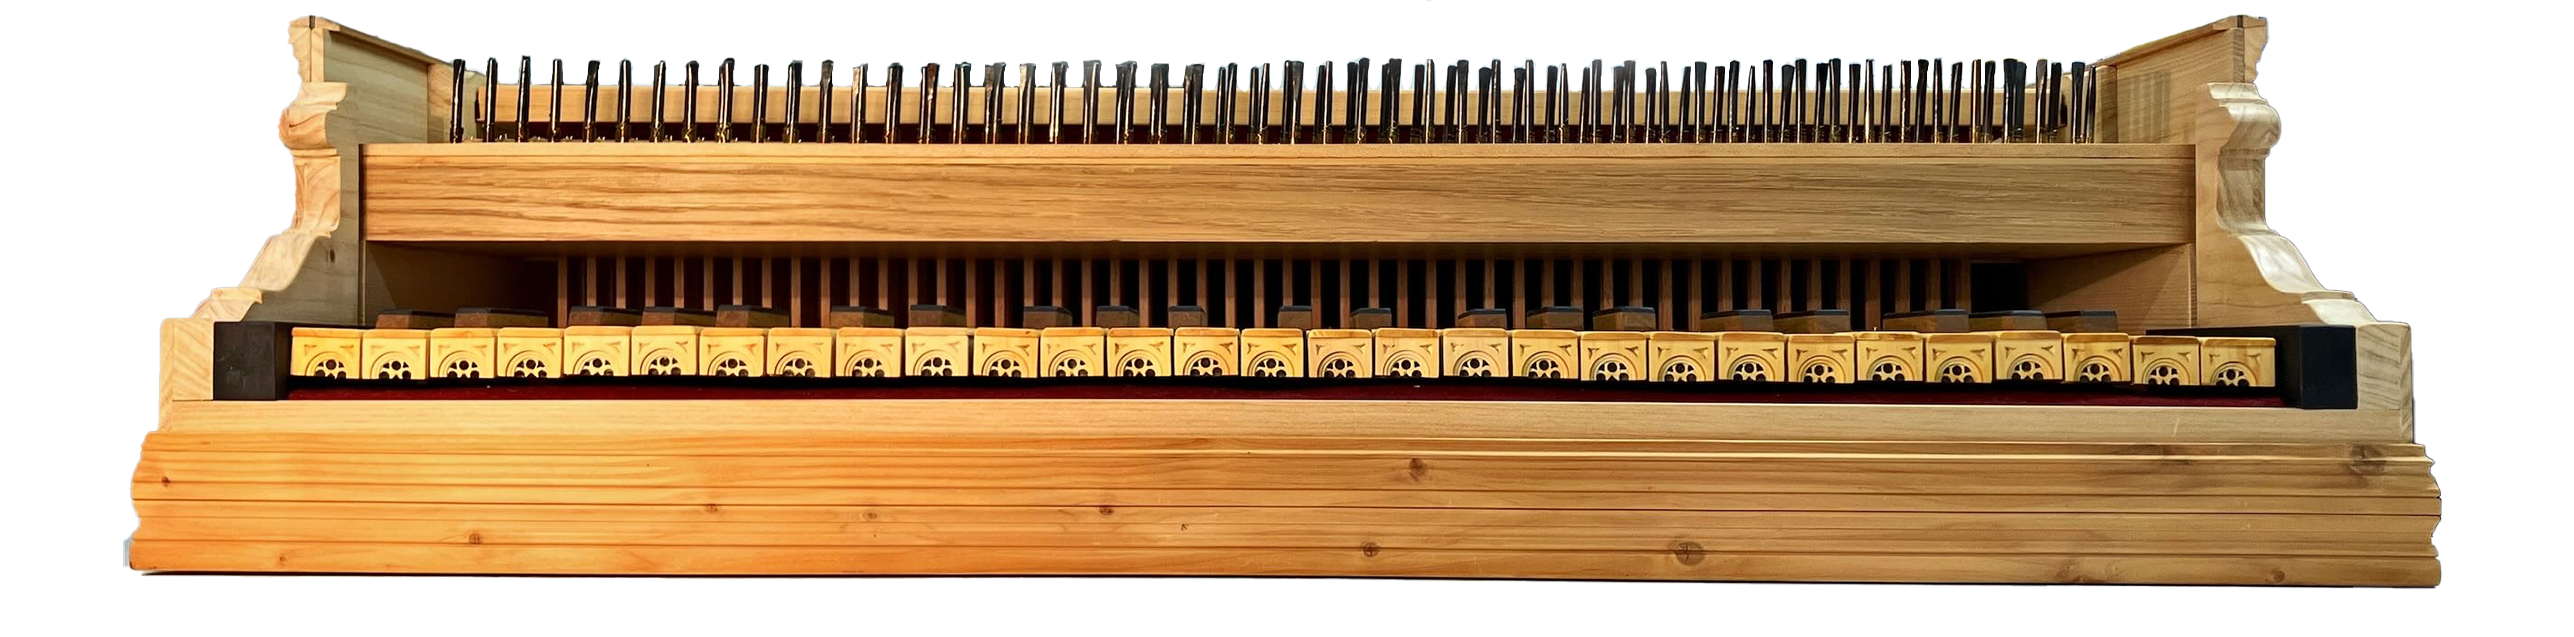
\includegraphics[width=\textwidth]{images/49-key-front.png}
%   \caption{49-key Model Harpsichord Mechanism by Roberto Livi, Bologna 2024}
%   \Description{49-key Model Harpsichord Mechanism by Roberto Livi, Bologna 2024}
%   \label{fig:teaser}
% \end{teaserfigure}

% Option 2:
\begin{teaserfigure}
 \hspace*{0.6in}
  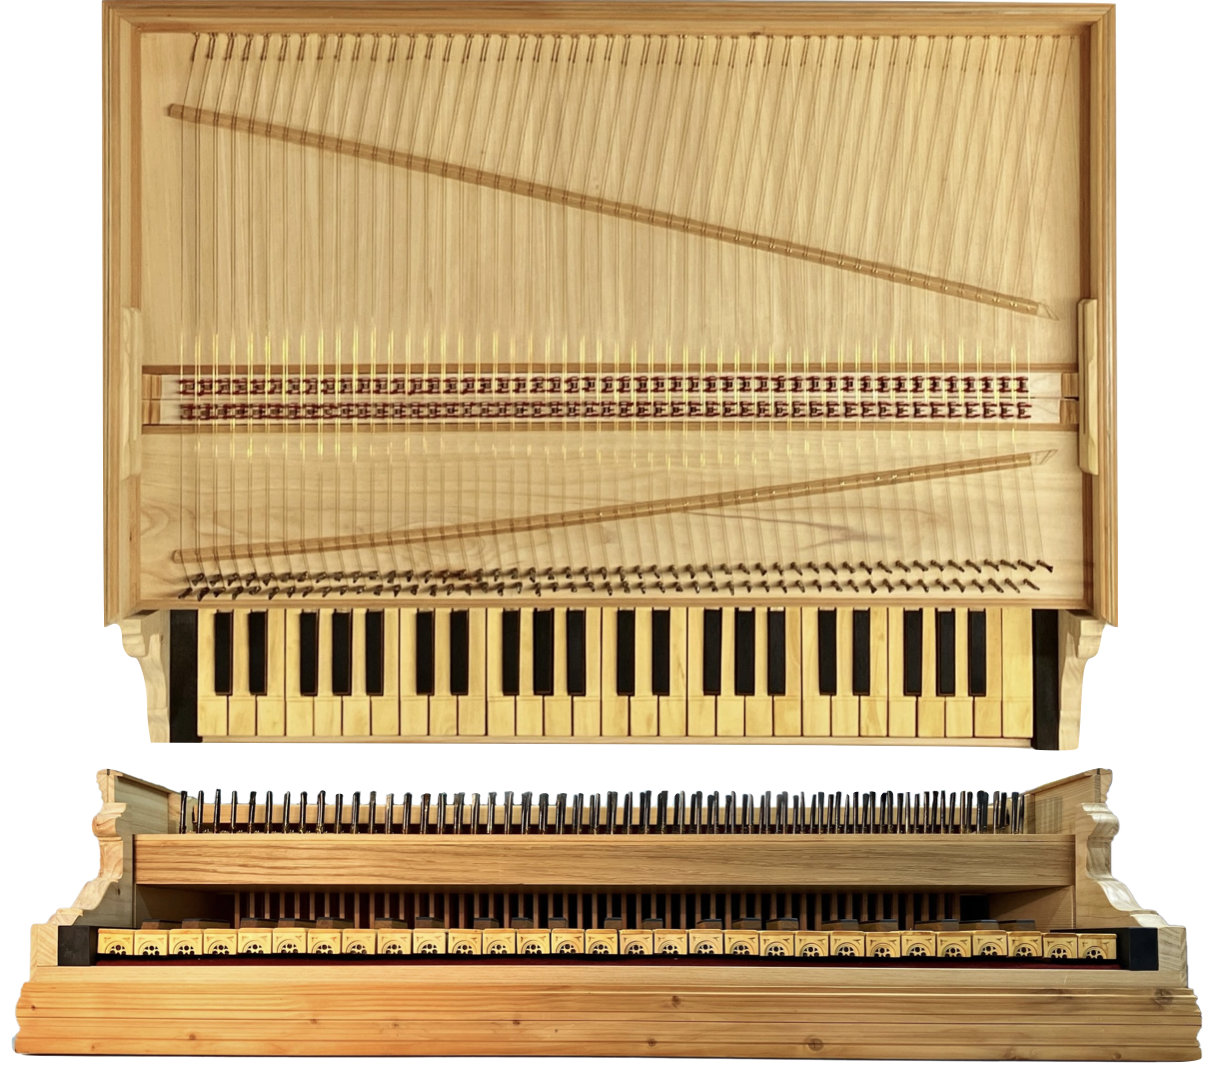
\includegraphics[width=0.8\textwidth]{src/images/49-key-front-top.png}
  \caption{49-key Model Harpsichord Mechanism by \anon{Roberto Livi, Bologna 2024}}
  \Description{49-key Model Harpsichord Mechanism by \anon{Roberto Livi, Bologna 2024}}
  \label{fig:teaser}
\end{teaserfigure}

% % Option 3:
% \begin{teaserfigure}
%   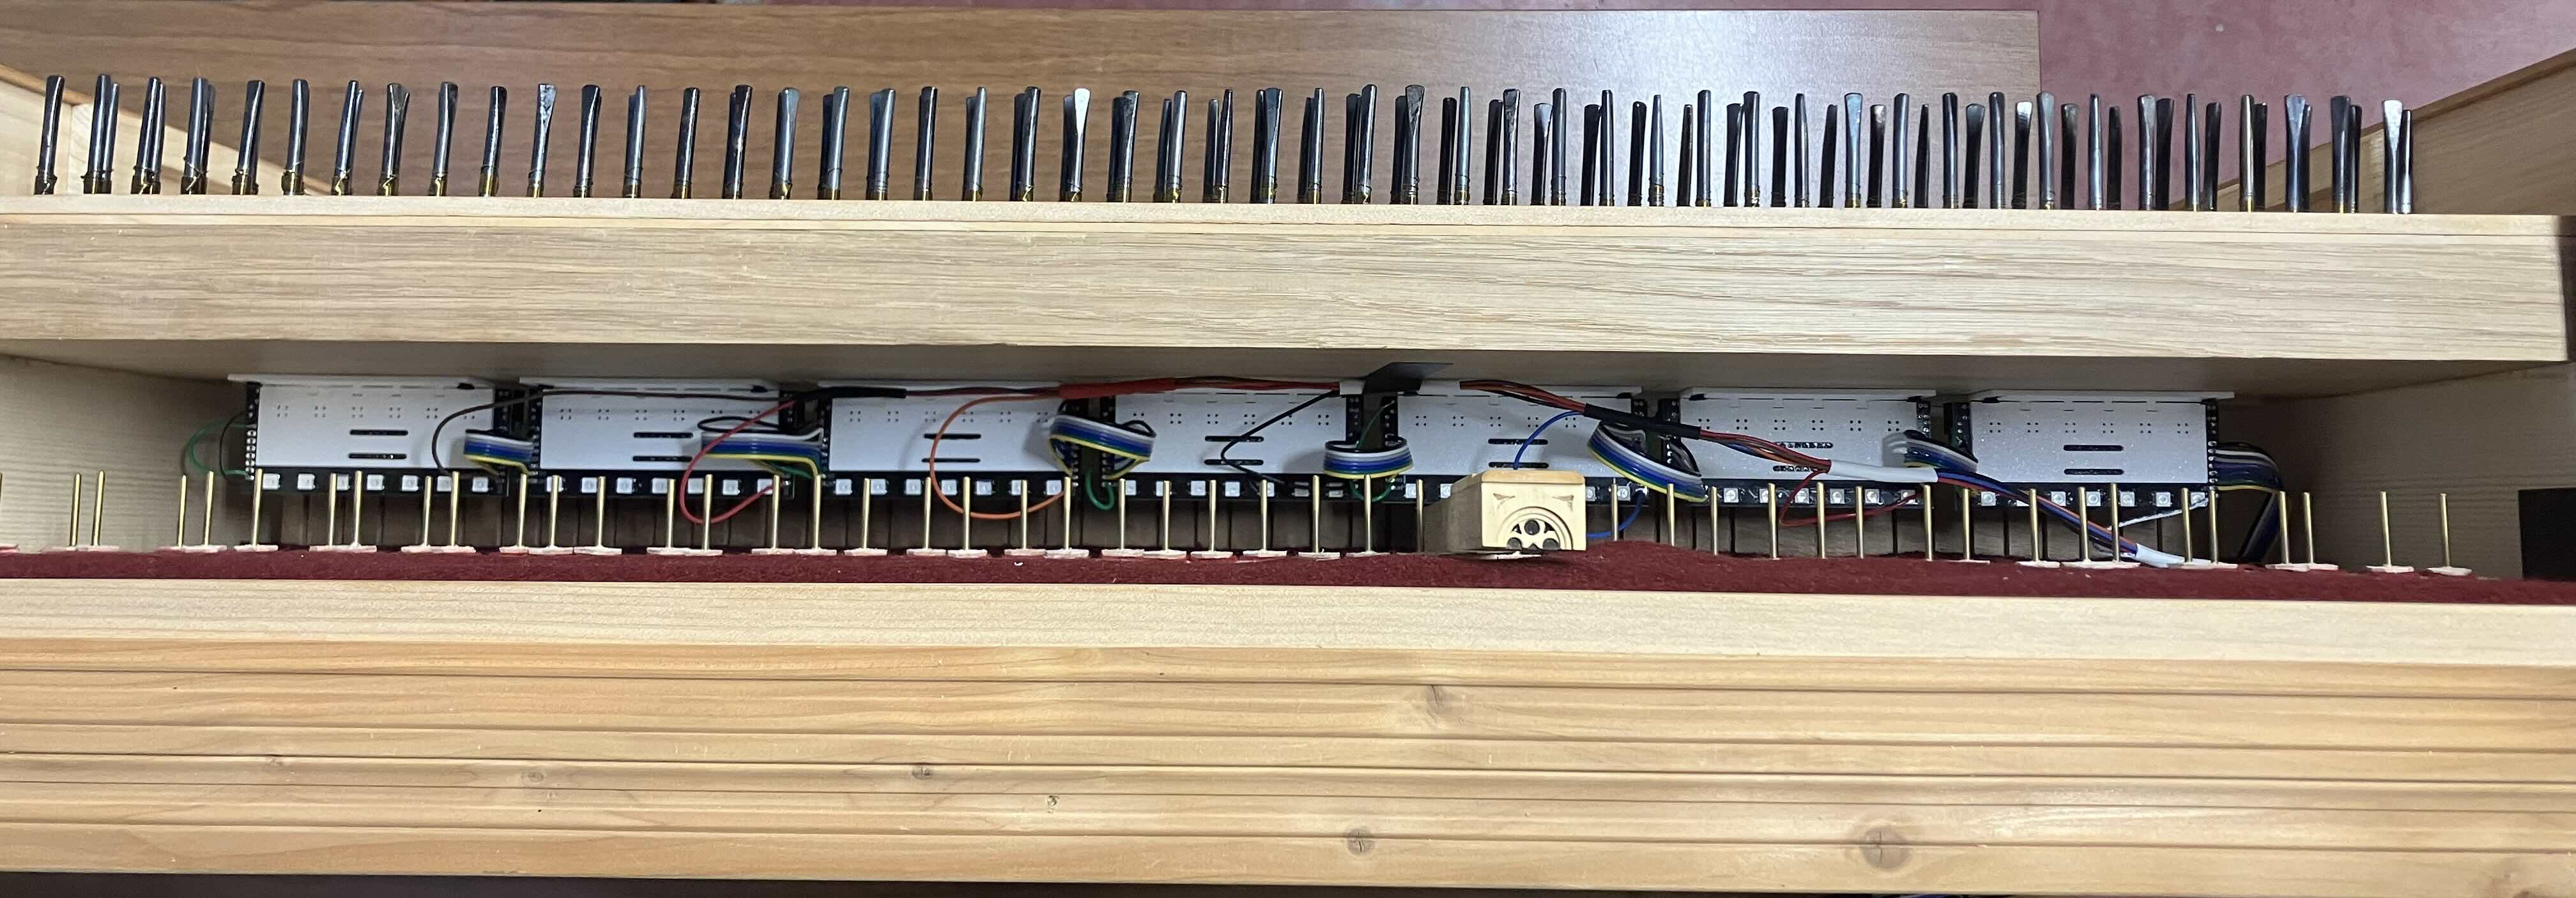
\includegraphics[width=\textwidth]{src/images/sensors-without-keys-front.jpg}
%   \caption{49-key Model Harpsichord Mechanism by Roberto Livi, Bologna 2024}
%   \Description{49-key Model Harpsichord Mechanism by Roberto Livi, Bologna 2024}
%   \label{fig:teaser}
% \end{teaserfigure}

%% Placeholder
% \begin{teaserfigure}
%   \includegraphics[width=\textwidth]{images/side_w-o_sensors.png}
%   \caption{3-key Model Harpsichord Mechanism by Graziano Bandini, Bologna 2023}
%   \Description{3-key Model Harpsichord Mechanism by Graziano Bandini, Bologna 2023}
%   \label{fig:teaser}
% \end{teaserfigure}

%%
%% This command processes the author and affiliation and title
%% information and builds the first part of the formatted document.
\maketitle

\section{Introduction}\label{introduction}

Technological advances have transformed how museums document, present and interpret their collections, fostering immersive experiences through tools such as laser scanning, 3D printing, and virtual reality \cite{allard2005use,Wachowiak01082009,RCM_2024_3D,Kuzminsky_LaserScan_2012,Schaich_3D_2007}. These technologies emphasise experiential authenticity, enabling encounters that evoke the past's sensory, emotional, and intellectual essence \cite{trant_Auth_1999}. However, as Pine and Gilmore note \cite{pinegilmore_2007}, achieving authenticity requires museums to navigate the delicate balance between preservation and meaningful engagement—a challenge that is particularly evident in the case of historical musical instrument collections \cite{McAlpine2014}.

Musical instruments represent a distinctive fusion of form, function, and history. Their cultural value extends beyond their visual appeal to include the tactile and auditory dimensions of use \cite{Fritz2017}. Yet, preservation concerns often limit direct interaction, reducing these artefacts to static displays. This ``red velvet cord'' approach, as theorised by McAlpine \cite{McAlpine2014}, protects fragile mechanisms but diminishes the instruments’ functional identity, disconnecting visitors from the full richness of their historical and cultural context.

The Tagliavini Collection in Bologna \cite{Tagliavini2007}, renowned for its historical keyboard instruments, exemplifies this dilemma. To address it, this project introduces an augmented replica of a historical harpsichord keyboard. 
% The project builds on an existing design borrowed from \cite{McPherson2013} and aligns with principles outlined in \cite{Masu_NIME_2023}, emphasising the importance of extending the lifecycle of existing NIMEs. 
The project fosters and complements the augmented piano keyboard design presented by McPherson \cite{McPherson2013} and ensures the relevance of previous NIME designs beyond their original context \cite{Masu_NIME_2023}. 


The article is organised as follows: TBC



\section{Related Work and Motivations}\label{related-work}


Museums often face significant challenges in engaging visitors due to limitations in staffing and funding, which restrict how visitors can interact with collections \cite{Templeton2018, McAlpine2014}. For musical instrument museums, these challenges are compounded by the difficulty of preserving historical instruments in a playable condition \cite{McAlpine2014}. The instruments' inherent fragility and gradual decay inevitably result in a point where they can no longer be played, even when collections adhere to the strictest conservation protocols \cite{NYT_strad}. A significant cultural change has taken place in recent decades, shifting the focus from the playability of the originals to their conservation. Karp \cite{Karp1979,Karp1985} advocates for a deeper understanding of musical instruments so that enough knowledge is generated to make them as ``copyable'' as possible.

McAlpine discusses a case similar to the Tagliavini collection in his examination of the Benton Fletcher Collection at National Trust Fenton House \cite{McAlpine2014}. When these instruments were donated, Benton Fletcher stipulated that they remain playable and should continue to be maintained for tuition and public performance. A large sampling campaign was conducted, and a custom MIDI interface was designed to fulfil this requirement while preserving the original instruments' integrity. The MIDI keyboard, comprising two commercially available keyboards mimicking the two-manual harpsichord layout, was used by visitors to trigger the instrument samples recorded with tailored strategies for each. However, user tests identified a significant limitation: the commercially available weighted keys failed to provide an authentic sense of interacting with a historical keyboard \cite{McAlpine2014}. 

On the other hand, the ``Tromba Moderna'' project \cite{Baldwin2016}, a previous NIME initiative, approached the issue of musical heritage playability by recreating and augmenting a replica of a historical tromba marina. A piezo transducer was connected to a sound synthesis engine and a driver within the instrument to simulate the expected vibrations of a historical tromba marina. 

This work inherits the same philosophy as the Tromba Moderna project. By augmenting a replica of a historical harpsichord keyboard using minimally invasive electronics and controlling a MIDI-triggered sample library, the project intends to offer a tool enhancing the fruition of the Tagliavini collection whilst retaining a form of continuity with historical instrument-building traditions. Furthermore, the electronics design borrows ideas from a previous NIME by McPherson \cite{McPherson2013}. As such, the interface proposed here is not, strictly speaking, a \emph{new} musical interface, particularly in its haptic response designed to adhere to longstanding harpsichord building traditions. However, this work complements and follows up on previous reflections regarding the \emph{sustainability of results} within the NIME community and identified as \emph{the O in NIME} \cite{Masu_NIME_2023}. The intended use of the keyboard through meaningful interaction with a museum exhibit is where the novelty of this work lies, rather than solely in its technological development. 

Beyond enhancing the visitor experience, future design iterations will serve as a research tool to explore the unique characteristics of the harpsichord and its impact on performance through the \anon{ERC-funded NEMUS} project, aiming to virtually reproduce the sound of historical keyboard instruments, and upcoming projects such as Rem@ke \cite{remake1}.

\section{Design Principles}\label{design}

\begin{figure*}
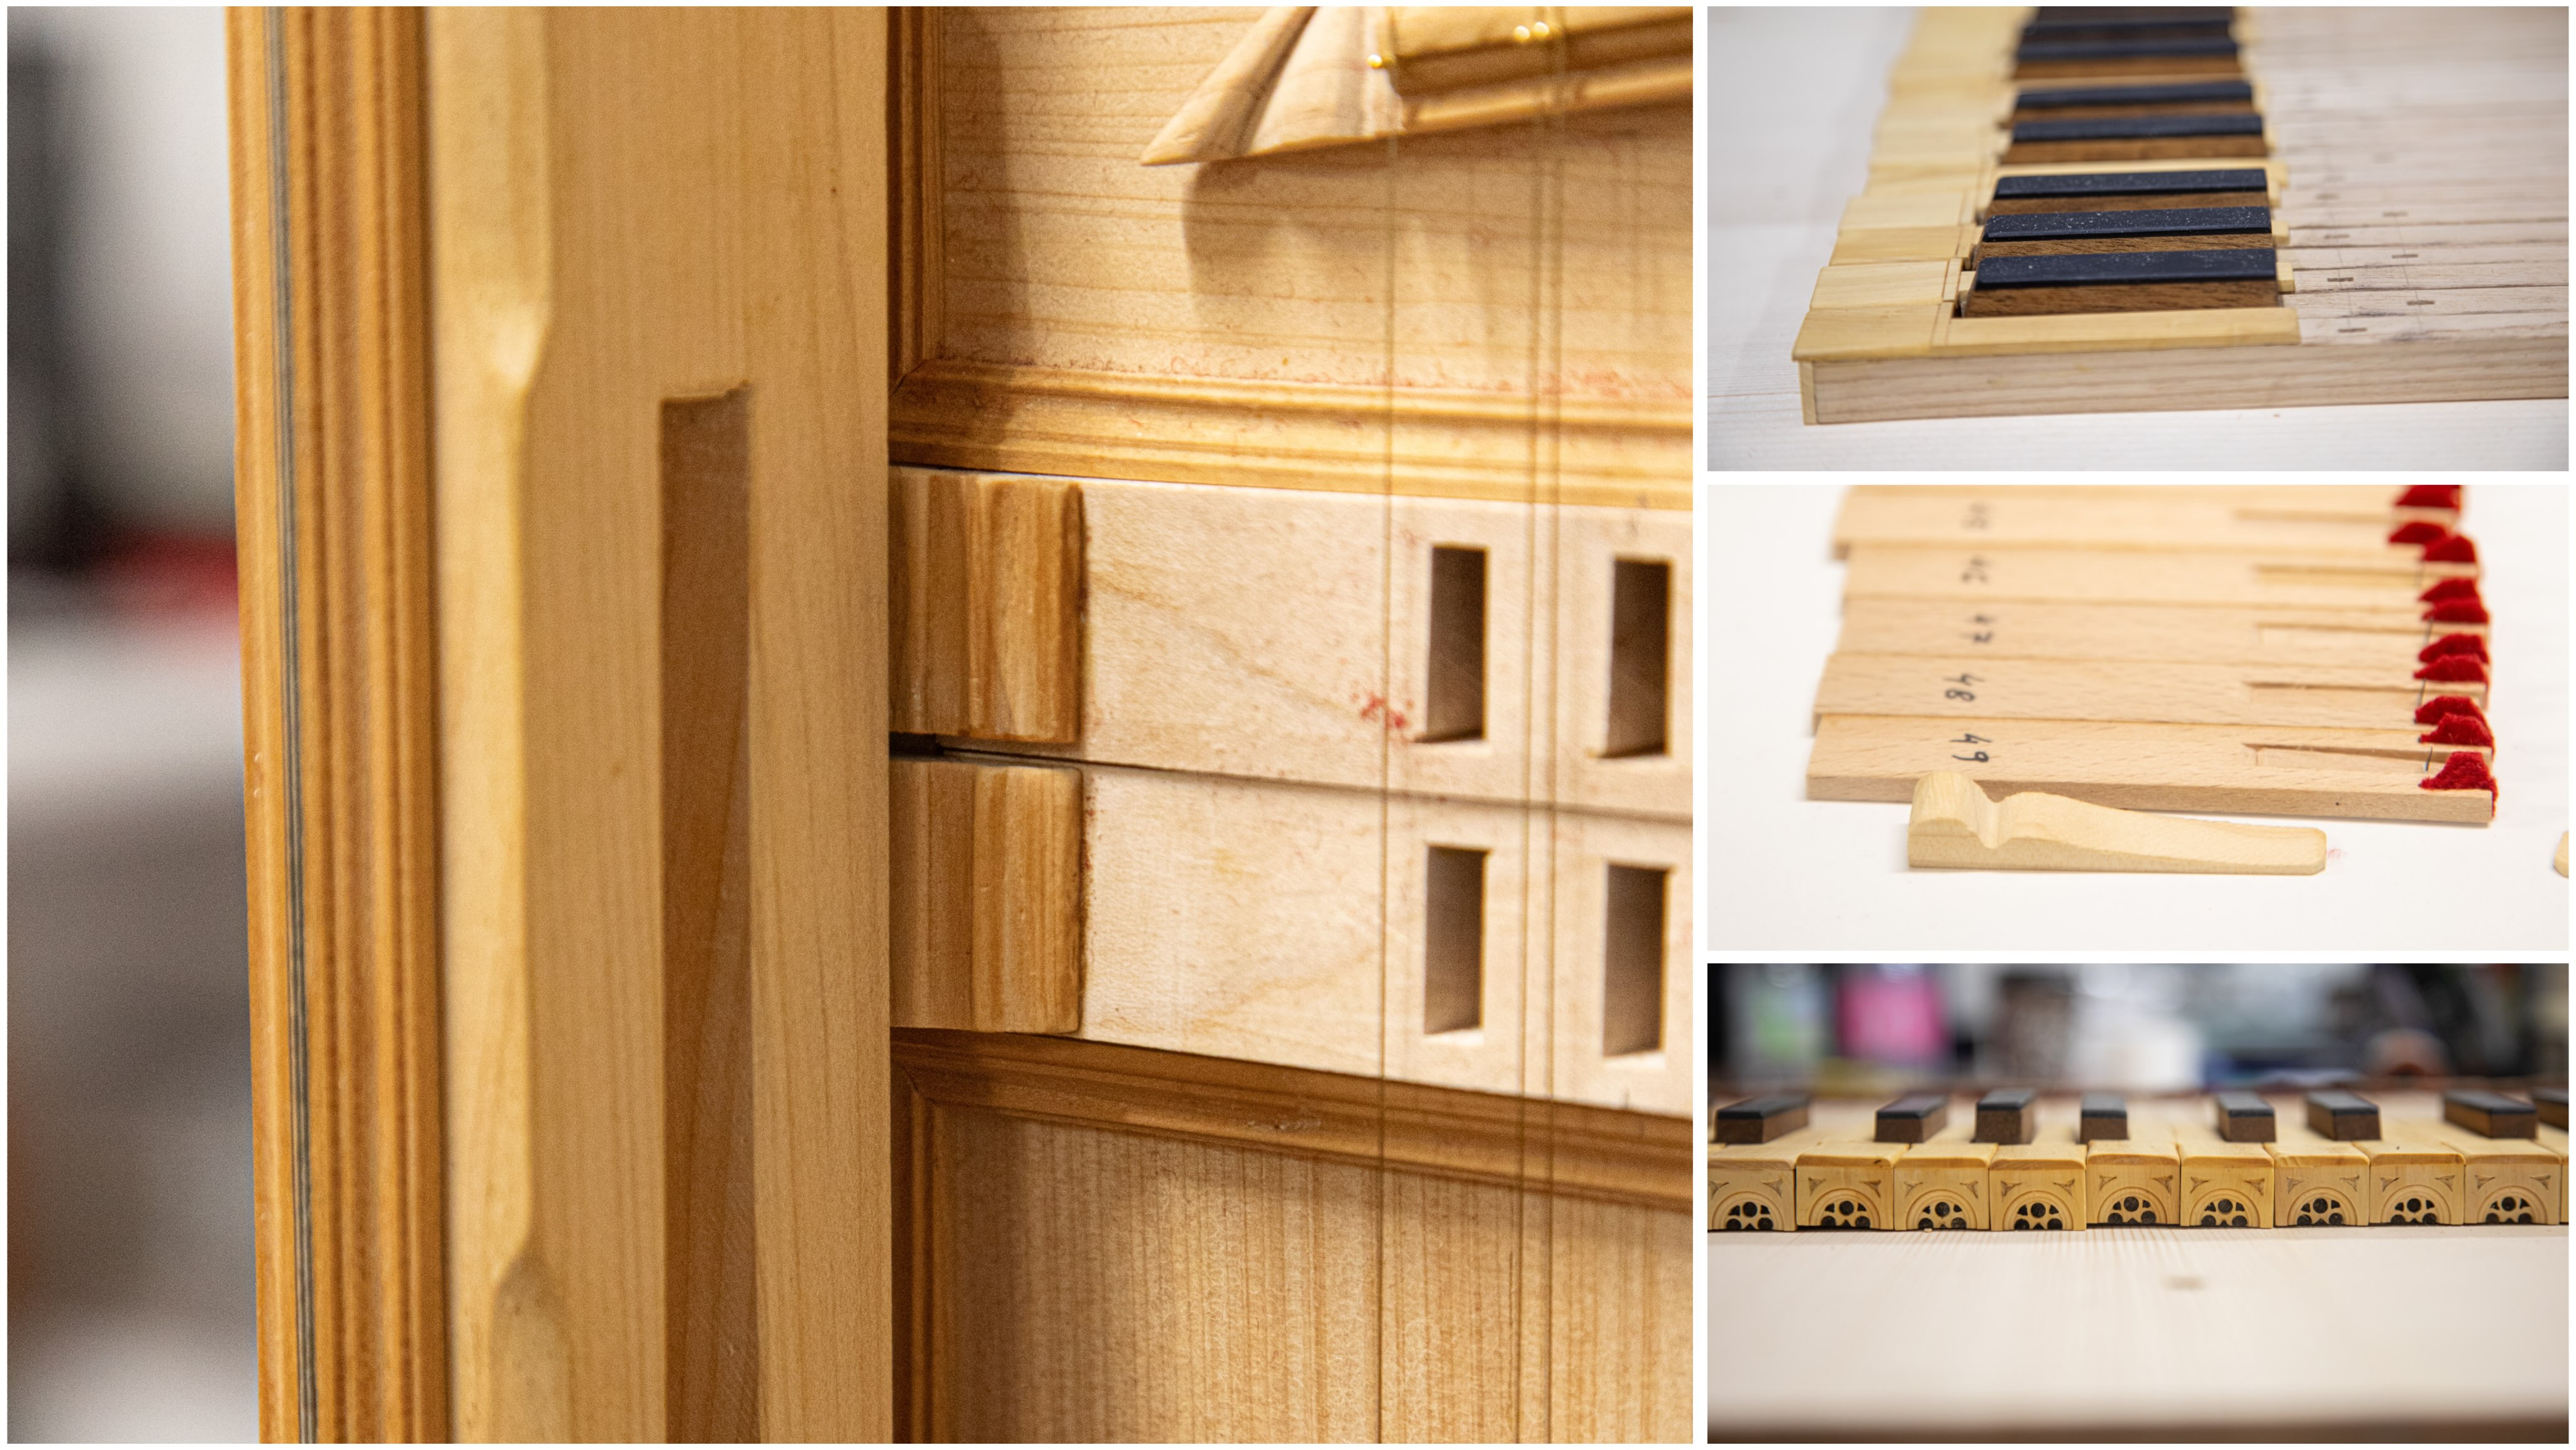
\includegraphics[width=\linewidth]{src/images/details.jpg}
\caption{Details of the replica, including the key slots and sides, keys, and jacks with seagull plectra.}\label{fig:details}
\end{figure*}

The design of the augmented replica keyboard for the Tagliavini Collection was guided by three principal constraints stipulated by the museum:
\begin{itemize}
\item \emph{No visible electronics}. To preserve the visual integrity of the exhibit, all electronic components had to remain concealed except for a pair of headphones and a small display for audio parameter adjustments.
\item \emph{Robustness and reliability}. The system needed to accommodate frequent use by museum visitors and allow for straightforward maintenance by staff without requiring specialised technical expertise.
\item \emph{Faithfulness}. The keyboard mechanism ensured fidelity to its authentic operation, keeping artefacts to a minimum. 
\end{itemize}
These constraints demanded a non-invasive, robust design that was respectful of the historical authenticity of the instruments. The requirement for faithfulness to the original mechanism immediately ruled out a mechanical design reliant on electromechanical actuators, as in previous works on piano haptics \cite{Timmermans2020,Gillespie1996}. While actuators can generate considerable force, they cannot replicate the wideband signals characteristic of the harpsichord's sharp and responsive haptics (A REFERENCE WOULD BE GOOD HERE, ANY IDEAS?), which differ significantly from a piano.

Here is a consolidated **Open-Source Design** subsection for your article:


\subsection{Open-Source Design and Cost-Effectiveness}\label{susec:open-source}

A central objective of this project was to ensure accessibility and reproducibility by committing to an open-source approach for all hardware, software, and data. The commitment to open-sourcing encompassed all aspects of the system, including hardware schematics, firmware, and calibration data. Cost-effectiveness was a central consideration. For example, the system was initially developed for a 3-key prototype and successfully scaled to 49 keys without significant increases in cost or complexity. Key components, such as QRE1113 sensors and CD4051BE multiplexers, were selected for their affordability and availability, while the modular PCB design ensured efficient replication and maintenance.

The Arduino Nano BLE was chosen as the core microcontroller for its compatibility with open-source tools and its ability to support both USB and BLE MIDI. Ferroelectric RAM (FRAM) was employed for data storage, offering an economical yet robust solution for preserving calibration settings across power cycles. Calibration workflows were optimised using the Arduino IDE’s serial plotter and open-source MIDI Monitor software, reducing reliance on proprietary tools and simplifying the process for users.

Scalability and ease of assembly were prioritised throughout the design process. The modular structure of the PCBs, combined with 3D-printed baffles and gradient stickers, ensured that the system could be scaled up without compromising performance or cost-efficiency. Installation and calibration times were reduced through iterative improvements, such as the integration of addressable LEDs for sensor identification during setup. These design choices align with the project’s open-source ethos, allowing assembly using standard tools commonly available in university maker spaces.

By making the hardware and software openly available, the project invites contributions and adaptations from the broader community. This transparency supports critical evaluation and encourages iterative improvements, promoting sustainability and innovation in interactive musical interface design. Moreover, the emphasis on affordability and accessibility ensures that the system can be adopted by a wide range of users, from cultural heritage institutions to academic researchers, reinforcing the project’s commitment to democratising access to advanced technological solutions.


\subsection{Summary of the Finalised Design}

The final design, visible in Figures \ref{fig:teaser} and \ref{fig:details}, is a 49-key harpsichord replica equipped with an optical sensor system reading the amount of light reflected by gradient stickers applied to the jacks' sides. Several key features were implemented to address the project’s requirements:

\begin{itemize}
\item \emph{QRE1113 infrared sensors}. These sensors were selected for their non-invasive properties and precision, enabling the detection of jack displacement without requiring structural modifications to the keyboard mechanism.
\item \emph{Gradient stickers}. Greyscale gradient stickers were applied to each jack to allow the infrared sensors to make precise readings. This approach made calibration easier and enabled scalability from a 3-key prototype to the final 49-key design.
\item \emph{Jack baffles}. Custom-designed baffles, 3D printed from dark pigmented PLA to minimise infrared reflection, were installed around the jacks to prevent cross-talk between adjacent sensors and ensure reliable data capture.
\end{itemize}

\begin{figure}  
  \centering
  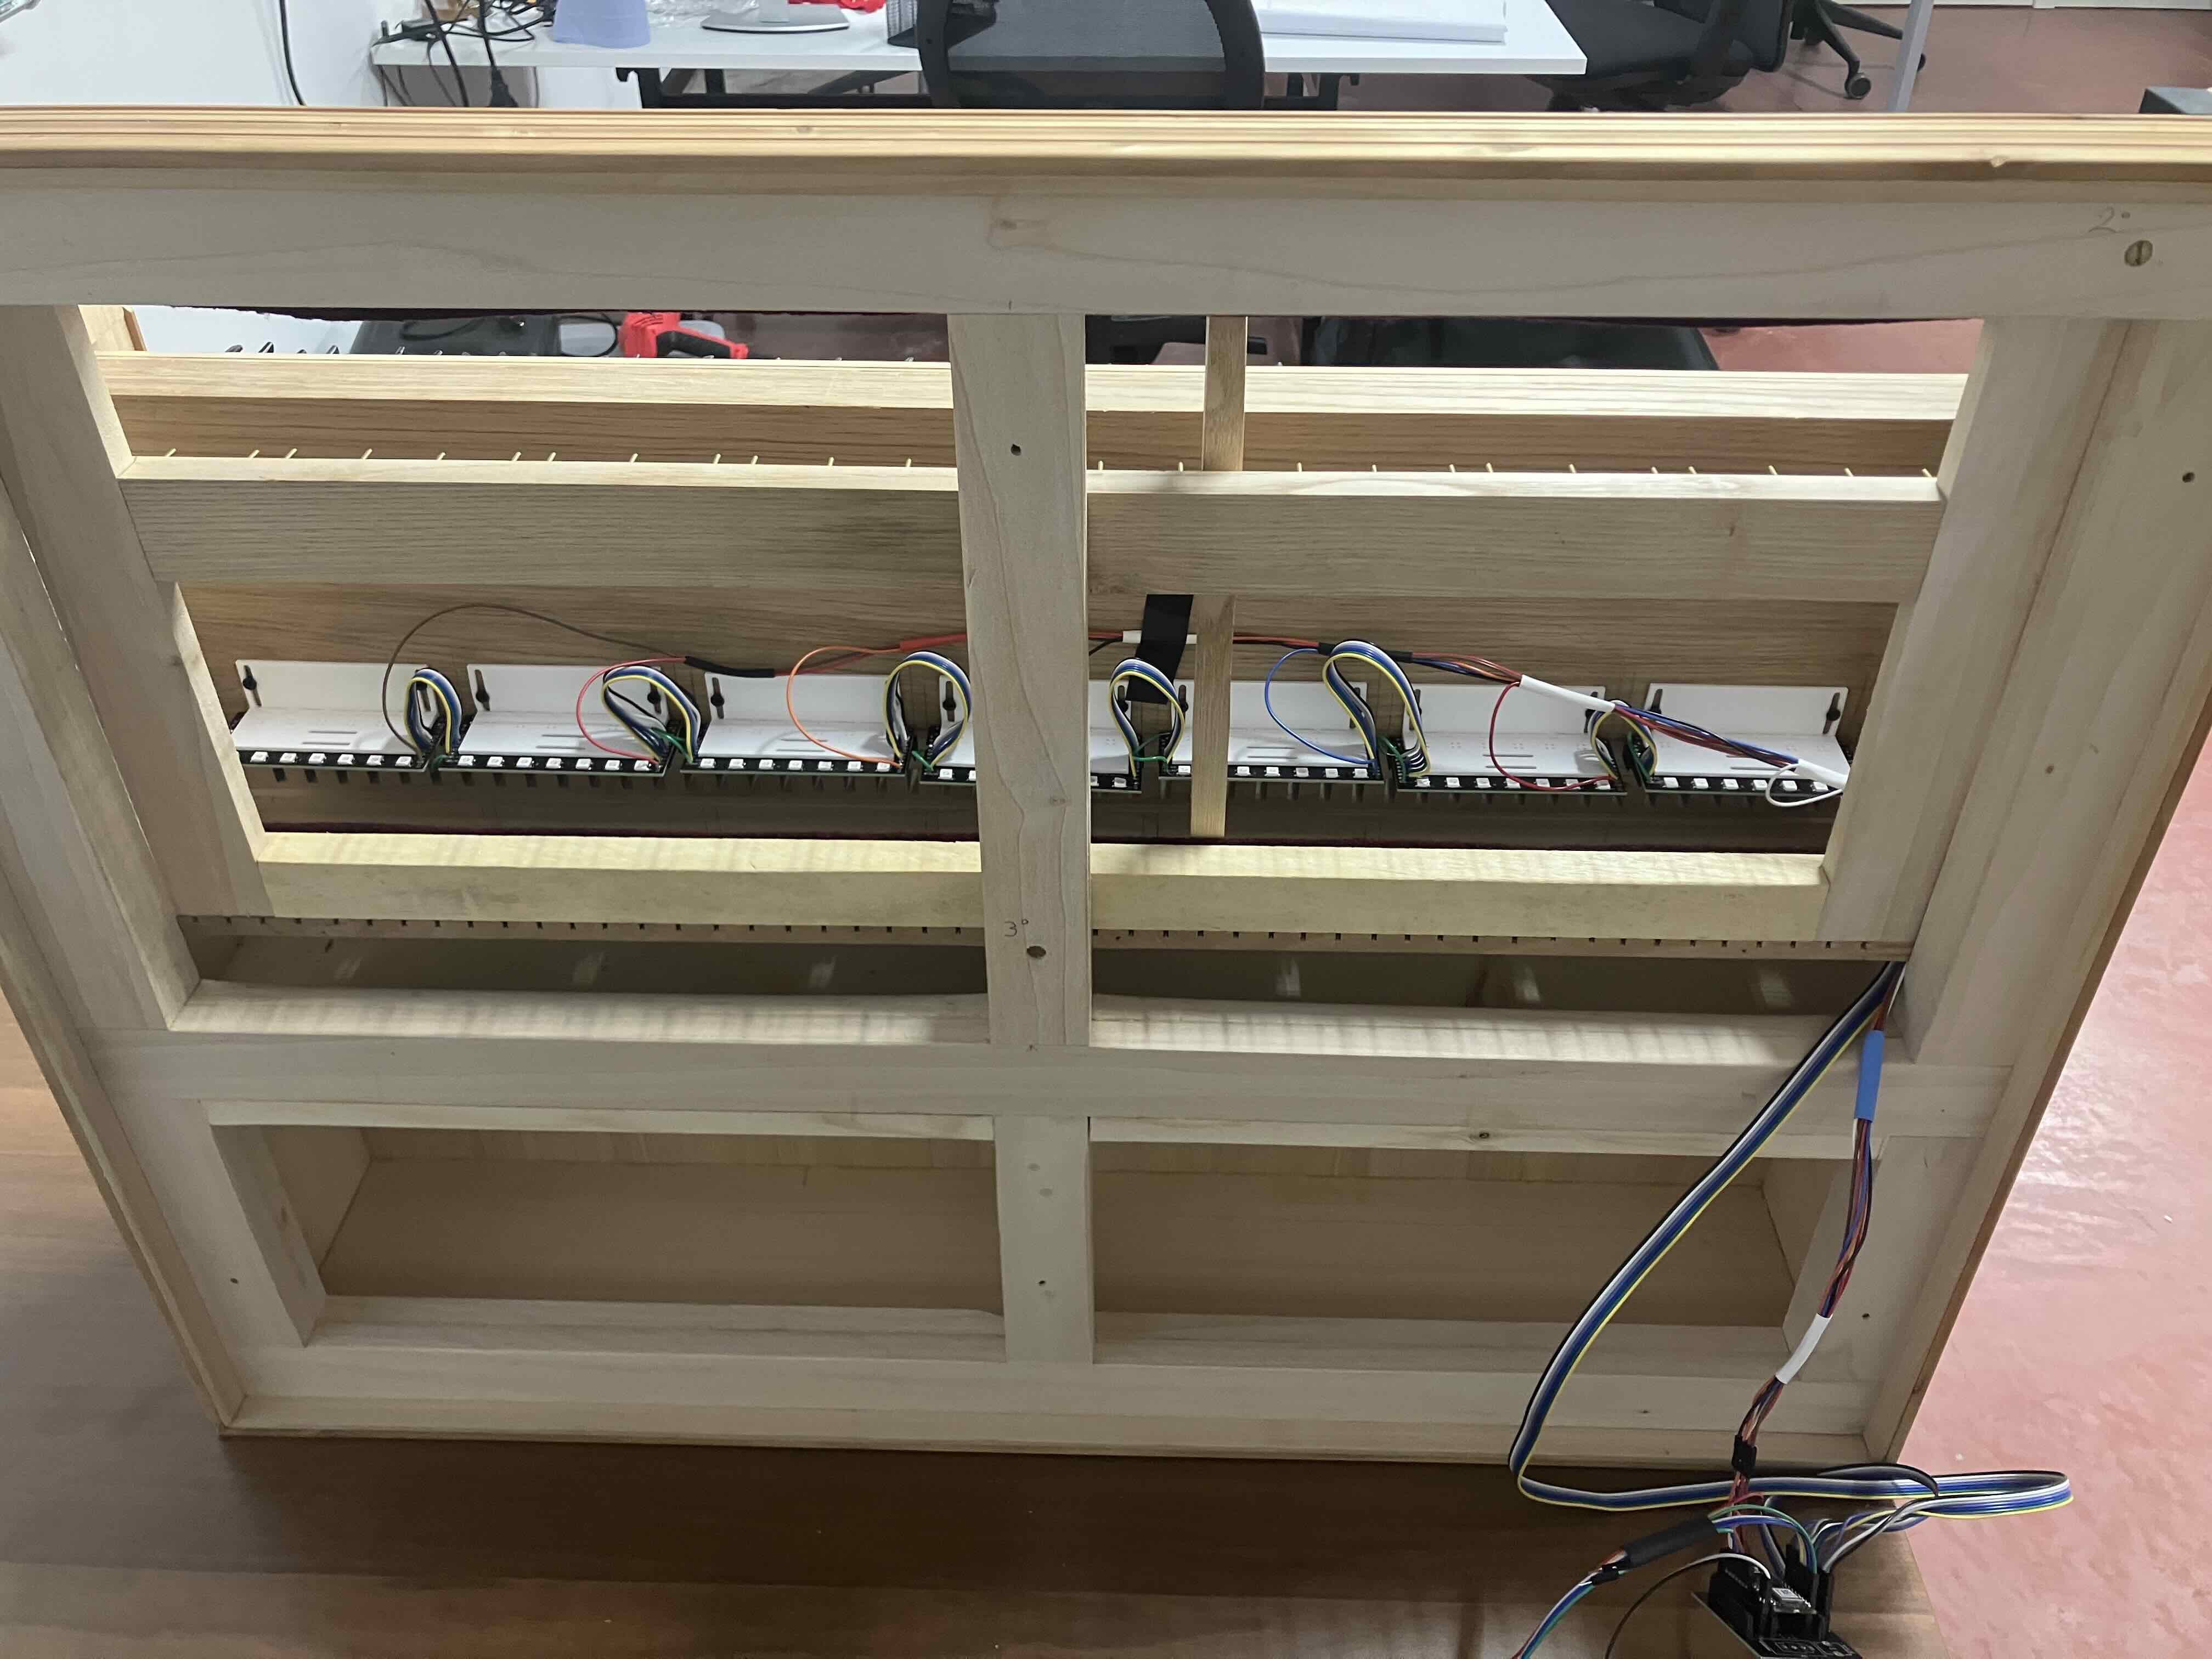
\includegraphics[width=\linewidth]{src/images/49-key-bottom-sensors-no-keys.jpg} 
  \caption{Underside of the full model keyboard, showing two chambers: the front chamber (top) and the rear chamber (bottom).} 
  \Description{} 
  \label{fig:49-key-bottom}
\end{figure}

A modular system of printed circuit boards (PCBs) was designed to manage the sensors and process their output. The 49 QRE1113 sensors were distributed across seven boards, containing 7 sensors each. The PCBs were secured to the underside of the keyboard mechanism, allowing them to be adjusted during installation. Ribbon cables connected the PCBs, providing flexibility during assembly while maintaining a compact form factor. Additional modifications, including baffles and adhesive improvements, were made to optimise the reliability of the sensor system during calibration and use.


The project built upon earlier NIME research on generating MIDI messages from piano keystrokes \cite{McPherson2013}, adapting it to address the unique characteristics of harpsichords and the specified constraints. Whereas the previous design emphasised continuous gesture tracking, this implementation required discrete key-triggered data to align with the needs of MIDI-triggered audio playback. 


\subsection{Materials and Construction}

The keyboard was designed to replicate the tactile and aesthetic sensations of playing an antique Italian harpsichord. Traditional materials were used, including walnut for the wrestplank, chestnut for the key levers, boxwood and ebony for key covers, and cypress for the case and soundboard. The 98 jacks were made from beech, fitted with brass springs and natural seagull feather plectra. The design was inspired by Venetian harpsichords, particularly the Alessandro Trasuntino instrument at the San Colombano Museum. 

The rectangular poplar frame deviates from the traditional logarithmic form to allow for the installation of the electronic sensors, as visible in Figure \ref{fig:49-key-bottom}, without compromising the visual or tactile authenticity. Two string orders, crafted from yellow brass wire and anchored with wrought iron pins, were tensioned to replicate authentic plucking resistance. Felt strips were added to dampen vibrations. The result is an interface that combines the mechanical action of keys with synthetic sound generation, preserving a real harpsichord's tactile and auditory qualities.


\section{Hardware Design}\label{hardware-design}

The hardware design aimed to fulfil the earlier constraints, including non-invasiveness, reliability, and scalability. To achieve these goals, the system evolved through iterative prototyping, beginning with simple threshold-based testing and culminating in a fully functional multi-sensor interface capable of triggering MIDI events.

\subsection{Prototyping and Key Model}

The initial stage of development focused on testing whether sensor data could reliably trigger MIDI playback. Modifying an existing harpsichord for testing was considered but ultimately discarded due to significant internal measurement and layout discrepancies. Instead, a custom 3-key harpsichord mechanism (Figure \ref{fig:3key}) was acquired from the museum and used as a foundation for prototyping. This approach followed a methodology similar to that used in Timmermans' Haptic Key project \cite{Timmermans2020}, enabling incremental validation of hardware and sensor integration.

The 3-key model facilitated iterative testing of individual components, including sensor placement, signal processing, and mechanical tolerances. The model’s compact form allowed for rapid experimentation while preserving the physical properties of a full-scale harpsichord.

\begin{figure}
    \centering
    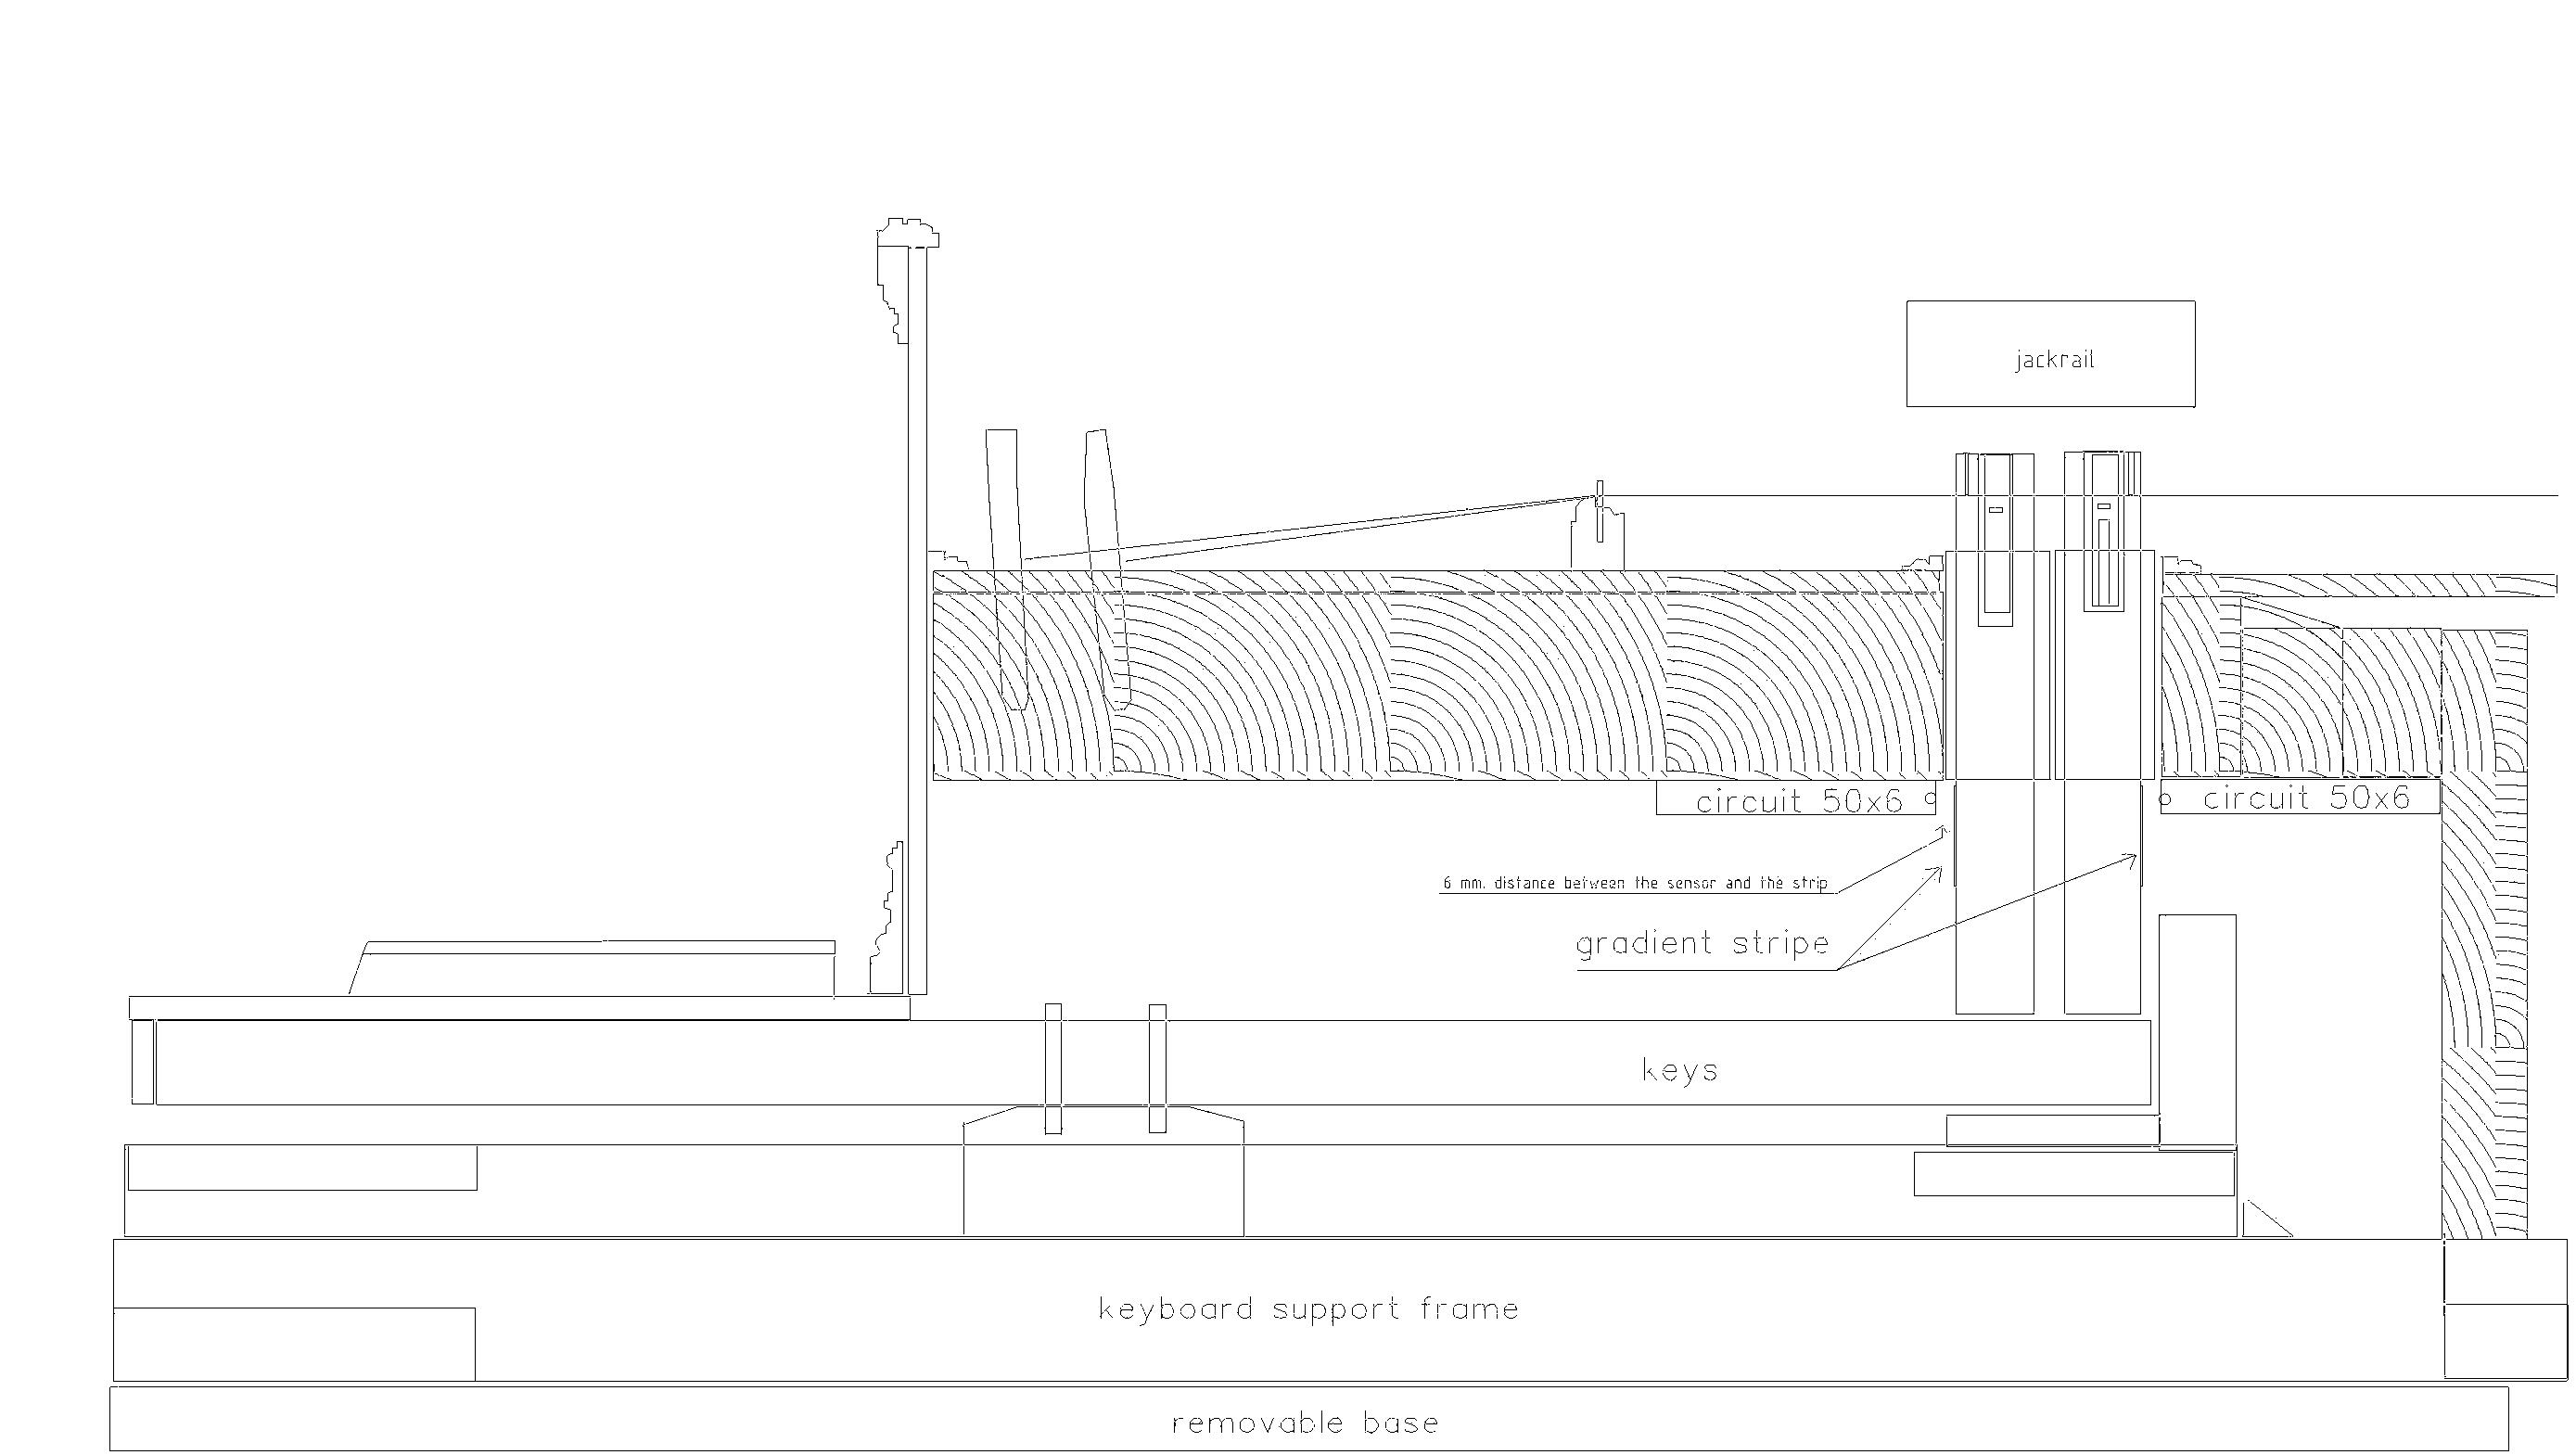
\includegraphics[width=\linewidth]{src/images/CrossSectionSensorPlacement.jpg}
    \\
    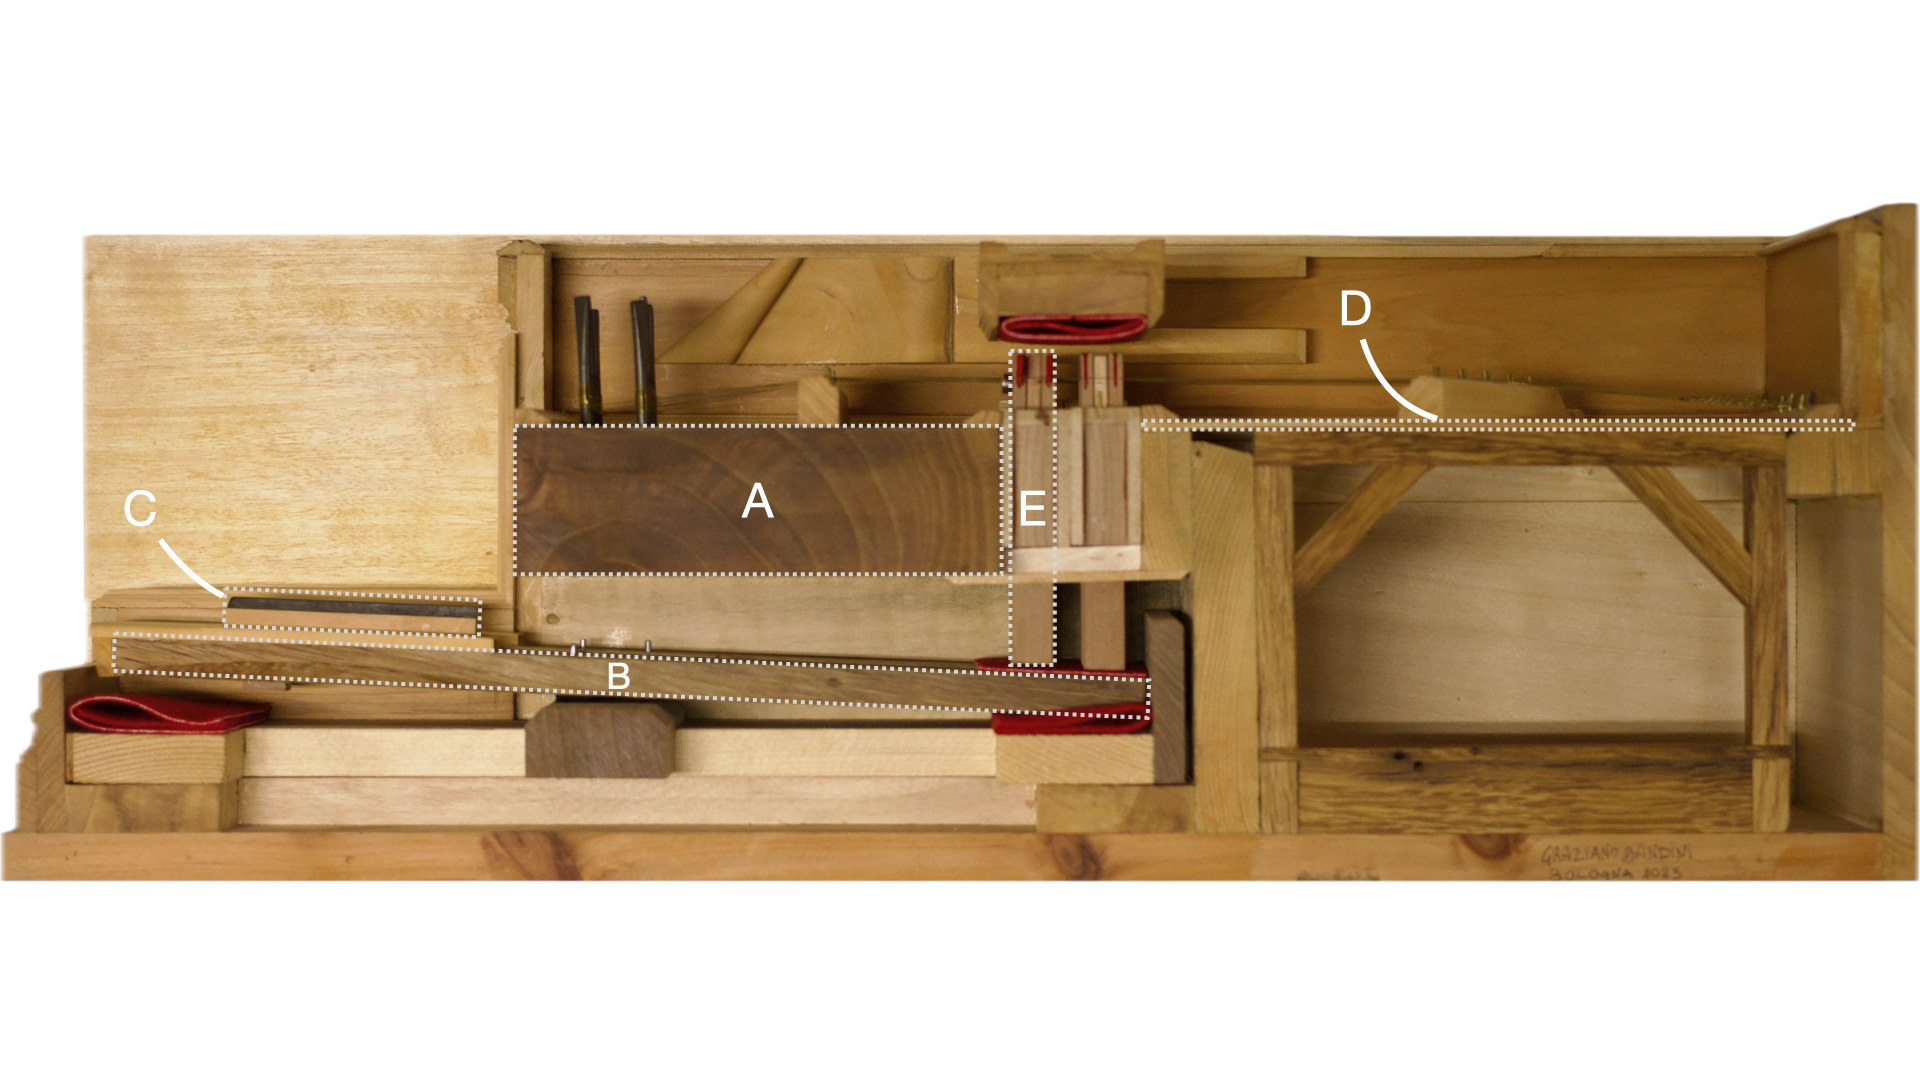
\includegraphics[width=\linewidth]{src/images/3-key-side-labelled.png}
    \caption{3-Key Model Harpsichord Mechanism designed by Graziano Bandini at San Colombano, Bologna, 2023. Key components include A: Wrestplank, B: Key Lever, C: Key Cap, D: Soundboard, E: Jack.}
    \label{fig:3key}
\end{figure}

% \begin{figure}
%     \centering
%        \begin{subfigure}
%          \centering
%          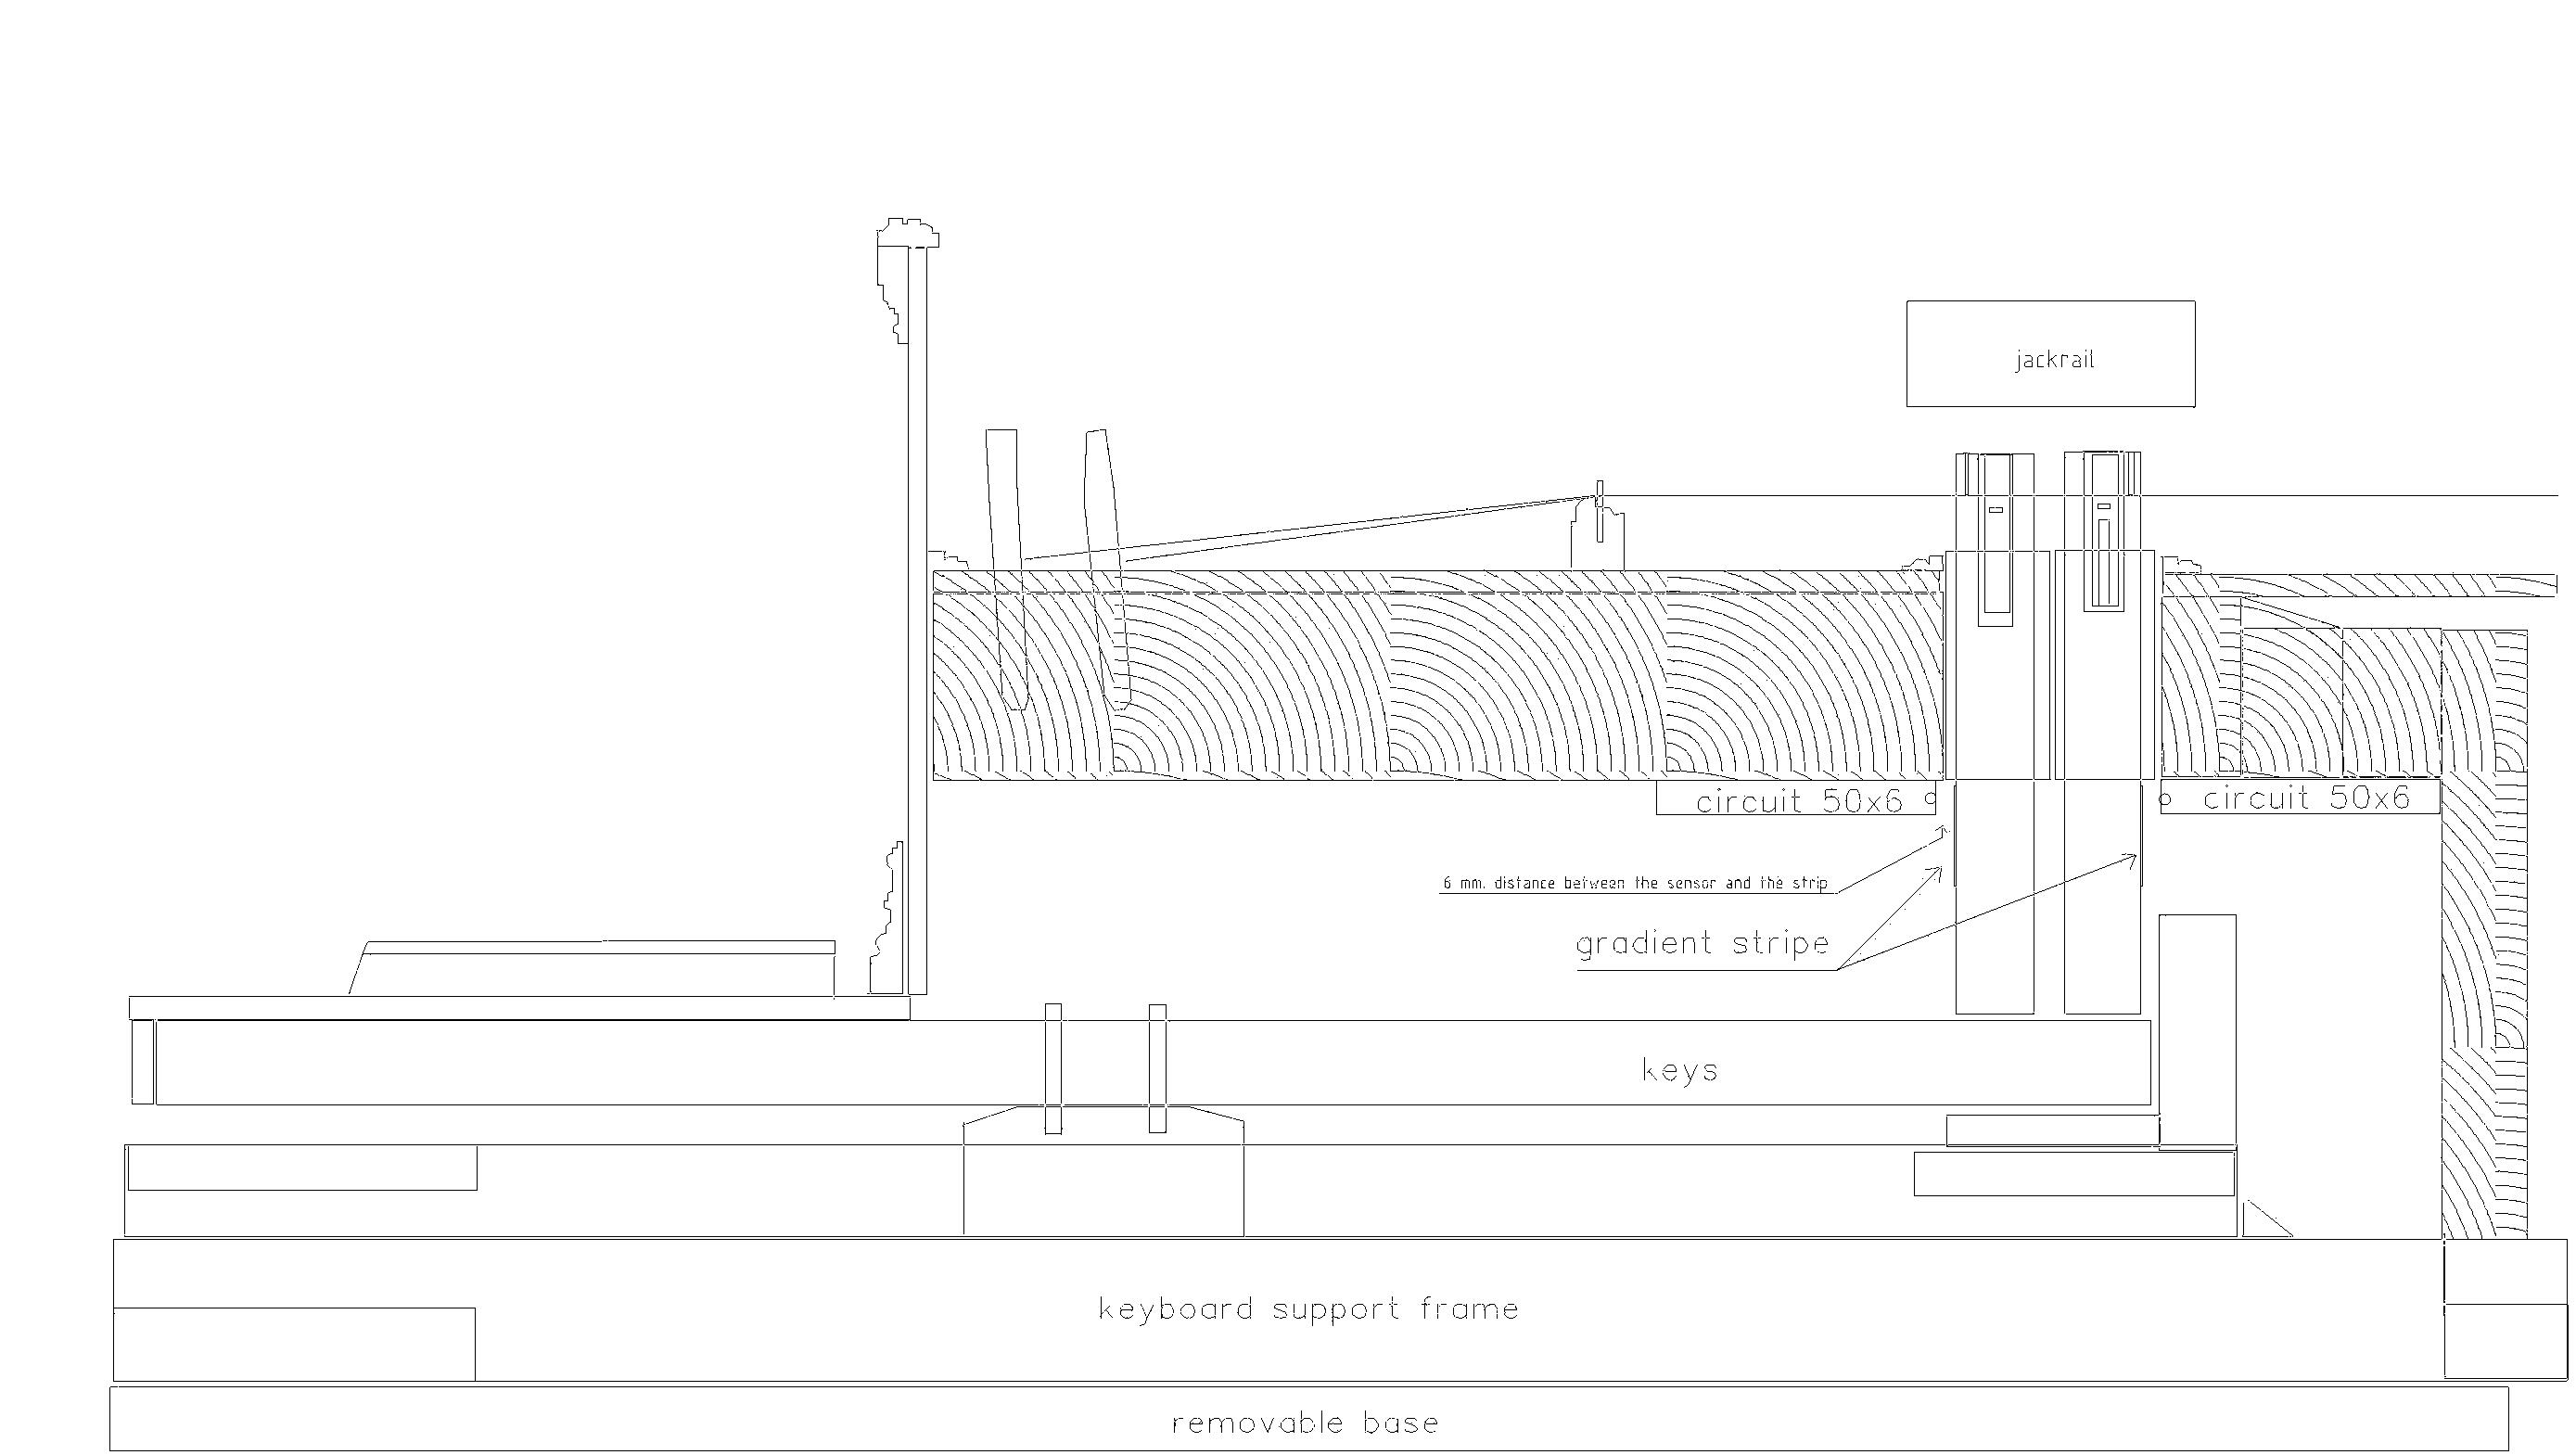
\includegraphics[width=\linewidth]{src/images/CrossSectionSensorPlacement.jpg}
%          \caption{Cross Section of 49-Key Model}
%          % \label{fig:y equals x}
%      \end{subfigure}\\
%     \begin{subfigure}
%          \centering
%          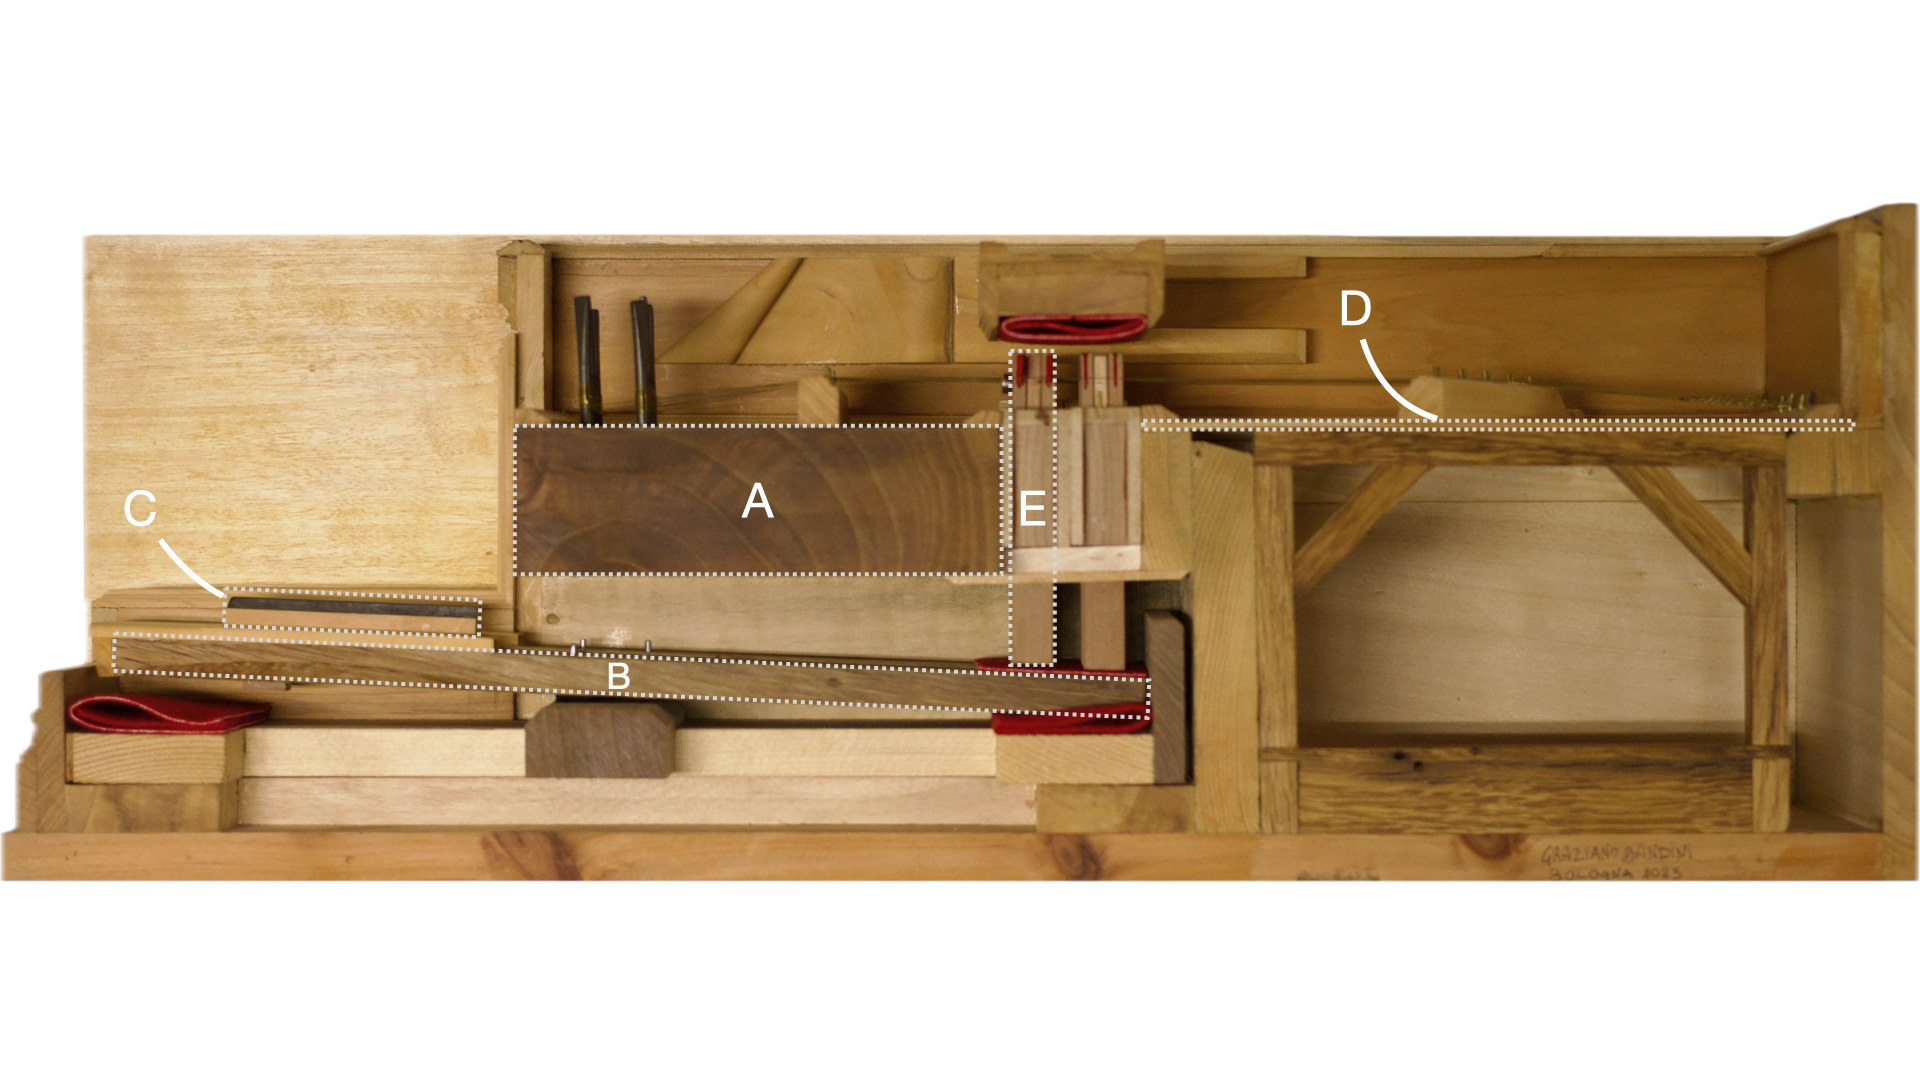
\includegraphics[width=\linewidth]{src/images/3-key-side-labelled.png}
%          \caption{3-Key Model: A: Wrestplank, B: Key Lever, C: Key Cap, D: Soundboard, E: Jack}
%          % \label{fig:y equals x}
%      \end{subfigure}        
%     \caption{Cross Sections of Models}
%     \label{fig:3key}
% \end{figure}

\subsection{Sensor Criteria}\label{sensor-criteria}

To ensure the system's suitability for a museum context, the following criteria were established to guide sensor selection and integration:

\begin{itemize}
    \item \emph{Non-invasive:} Sensors must not require significant modifications to the harpsichord's mechanical structure or aesthetics.
    \item \emph{Low Latency:} Sensor response times were required to remain under 10 ms, with an upper limit of 25 ms deemed acceptable \cite{Jack2016}.
    \item \emph{Reliability:} Sensor data had to be accurate, minimising false positives and negatives without excessive filtering.
    \item \emph{Scalability:} The design needed to be cost-effective and adaptable for up to 50 or more keys while maintaining consistent performance.
    \item \emph{Expandability:} The system should accommodate future functionality, such as additional MIDI parameters or data visualisation.
\end{itemize}

These criteria ensured that the design aligned with the open-source ethos of the project, allowing assembly in standard maker spaces without specialised equipment. 

\subsection{Sensor Board Design}\label{sensor-board}

\begin{figure*}
    \centering
    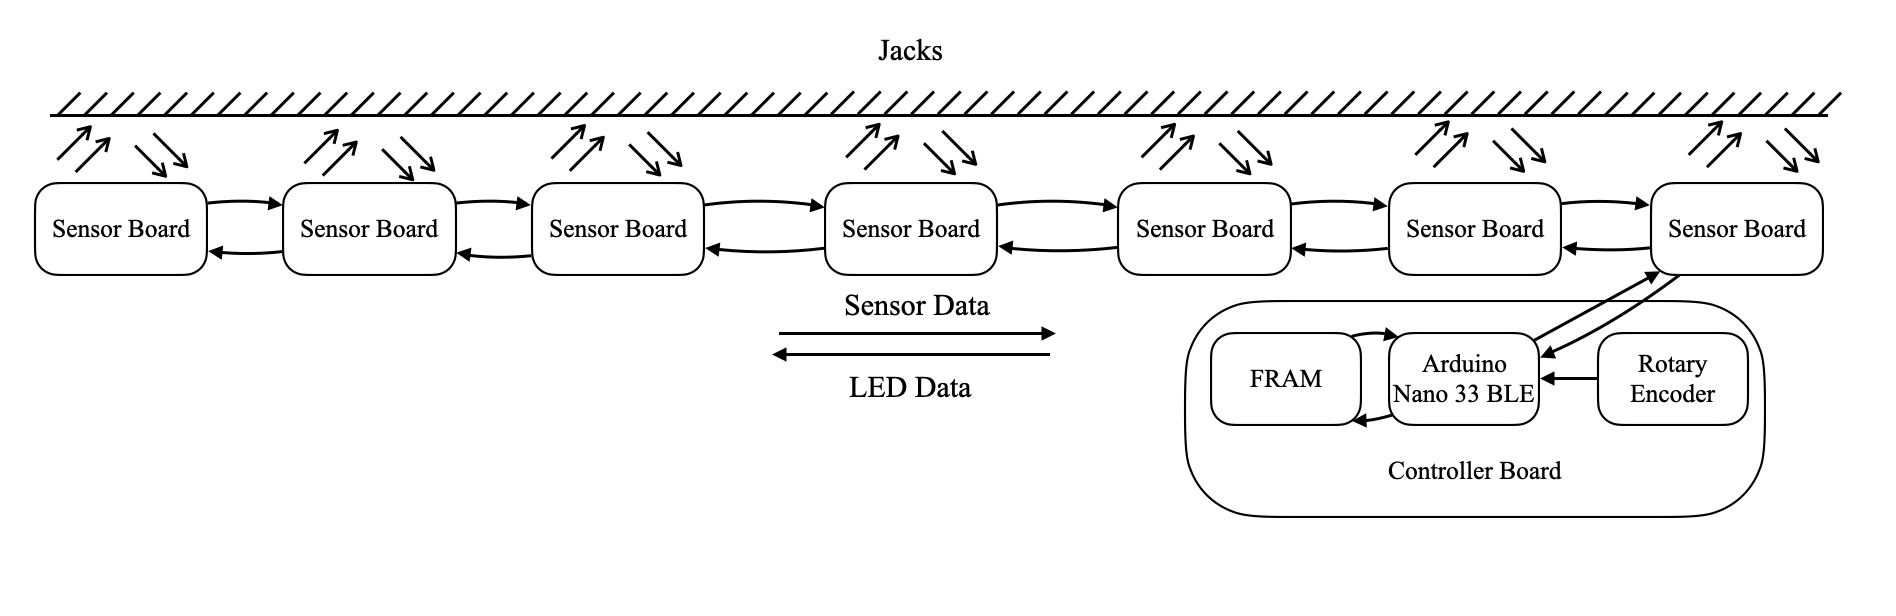
\includegraphics[width=\linewidth]{src/images/system-block-diagram-long.png}
    \caption{Block diagram of PCB connection. Sensor and LED are routed through each sensor PCB}
    \label{fig:system-block-diagram}
\end{figure*}

The final sensor system utilised QRE1113 infrared sensors, known for their precision and suitability for short-distance detection \cite{McPherson2013, McPherson2019}. The sensors were distributed across seven printed circuit boards (PCBs), each responsible for seven keys. Each PCB contained the following components:

\begin{itemize}
    \item 7 QRE1113 infrared sensors.
    \item 7 100 $\Omega$ resistors and 7 10 k$\Omega$ resistors (later reduced to one resistor per board).
    \item 1 Texas Instruments CD4051BE multiplexer for signal aggregation.
\end{itemize}

The QRE1113 sensors function by detecting infrared light reflected from nearby surfaces. The gradient stickers affixed to each jack provided a consistent reflective surface for the sensors, enabling precise tracking of jack displacement. This approach was chosen for its simplicity and scalability, allowing the design to progress from the 3-key prototype to a 49-key model without significant modifications.

To eliminate cross-talk between adjacent sensors, 3D-printed baffles were installed on the PCBs (Figure \ref{fig:baffles}). These baffles, fabricated from dark-pigmented PLA, ensured that infrared reflections from neighbouring jacks did not interfere with sensor readings. Testing confirmed that this measure significantly improved data reliability.

\begin{figure}  
  \centering
  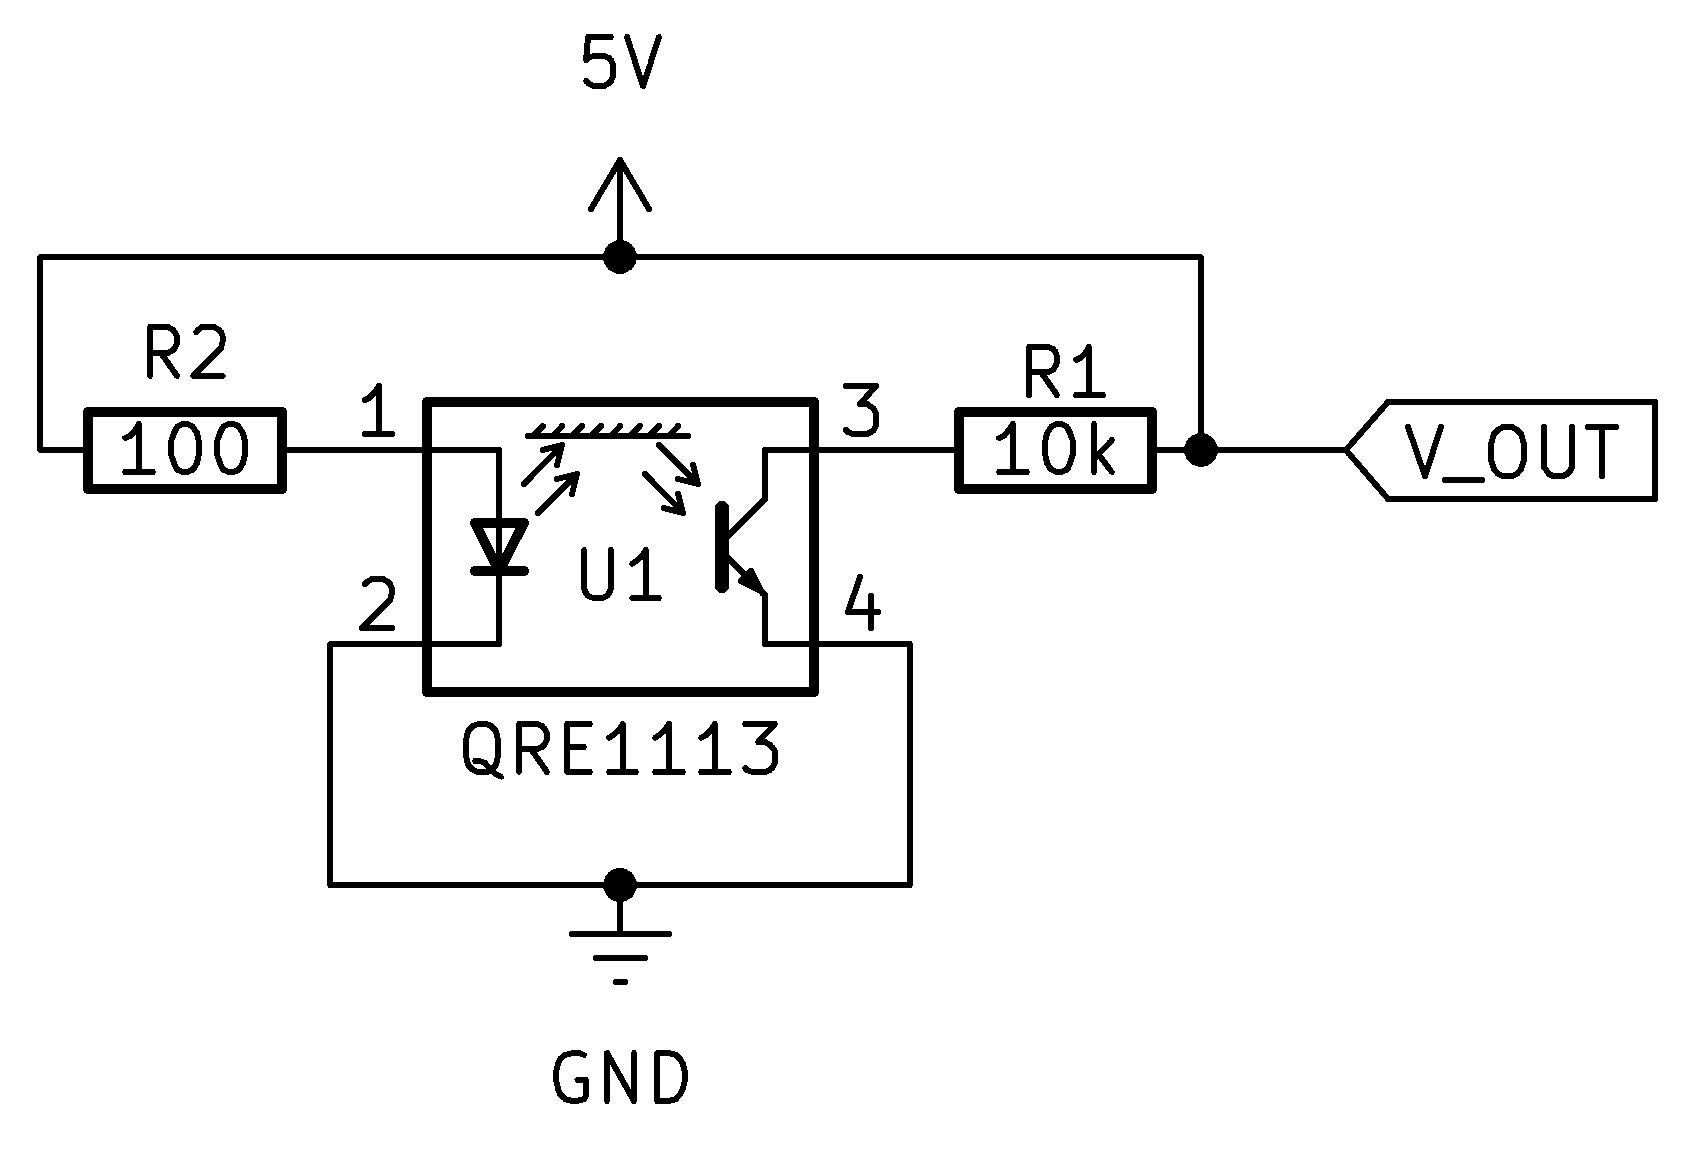
\includegraphics[width=\linewidth]{src/images/simple-schematic-bw-.jpg} 
  \caption{Optical sensor in a simple voltage divider circuit. \texttt{V\_OUT} is routed to one of 8 channels on the CD4051BE multiplexer}
  \Description{} 
  \label{fig:simple-schematic}
\end{figure}

\subsection{Controller Board}\label{controller-board}

The controller board, designed around the Arduino Nano BLE platform, was the central hub for processing sensor data and triggering MIDI messages. The Nano BLE was selected for its compact form factor, integrated BLE MIDI functionality, and native USB support. These features simplified development while ensuring compatibility with existing MIDI-based synthesis systems.

Initial iterations used 2.54 mm pitch headers for cable connections, but issues with cable disconnections led to the adoption of JST-PH connectors in later designs. Custom cable looms were constructed using adapted crimping tools, ensuring robust connections without compromising accessibility.

Non-volatile memory, implemented using Ferroelectric RAM (FRAM), provided a reliable means of storing calibration data. This ensured that sensor thresholds and other settings could be preserved across power cycles, enhancing the system's usability in museums.

\subsection{Calibration and Power Management}\label{calibration}

Each sensor's threshold was manually adjusted using RGB LEDs integrated into the system. These LEDs provided visual feedback during calibration, enabling the identification of malfunctioning sensors and simplifying the alignment process. The calibration workflow utilised the Arduino IDE serial plotter and open-source MIDI monitoring software (Figure \ref{fig:serial_monitor}). 


As an expert harpsichord performer, finer calibration was carried out with the guidance of \anon{Catalina Vincens}.

Power requirements for the system were estimated at 1.1 A at 5 V, with fluctuations during startup. While the sensors were powered continuously in this iteration, future designs may incorporate power-saving measures, such as dynamic activation of sensors based on usage.

\subsection{Final Assembly and Integration}

The final 49-key harpsichord replica incorporated the sensor and controller boards into a rectangular frame, deviating slightly from traditional designs to accommodate electronic components. Ribbon cables connected the PCBs, while felt strips were interwoven between the strings to suppress vibrations and maintain the tactile response of the keys.

The assembly process at the NEMUS lab in Bologna involved meticulous adjustments to key clearances and wiring layouts. Modifications included milling sections of the keys to ensure adequate clearance for the PCBs and varnishing the jacks to improve sticker adhesion. Subsequent iterations addressed these challenges, refining the system’s scalability and robustness.



% \begin{figure}
%     \centering
%     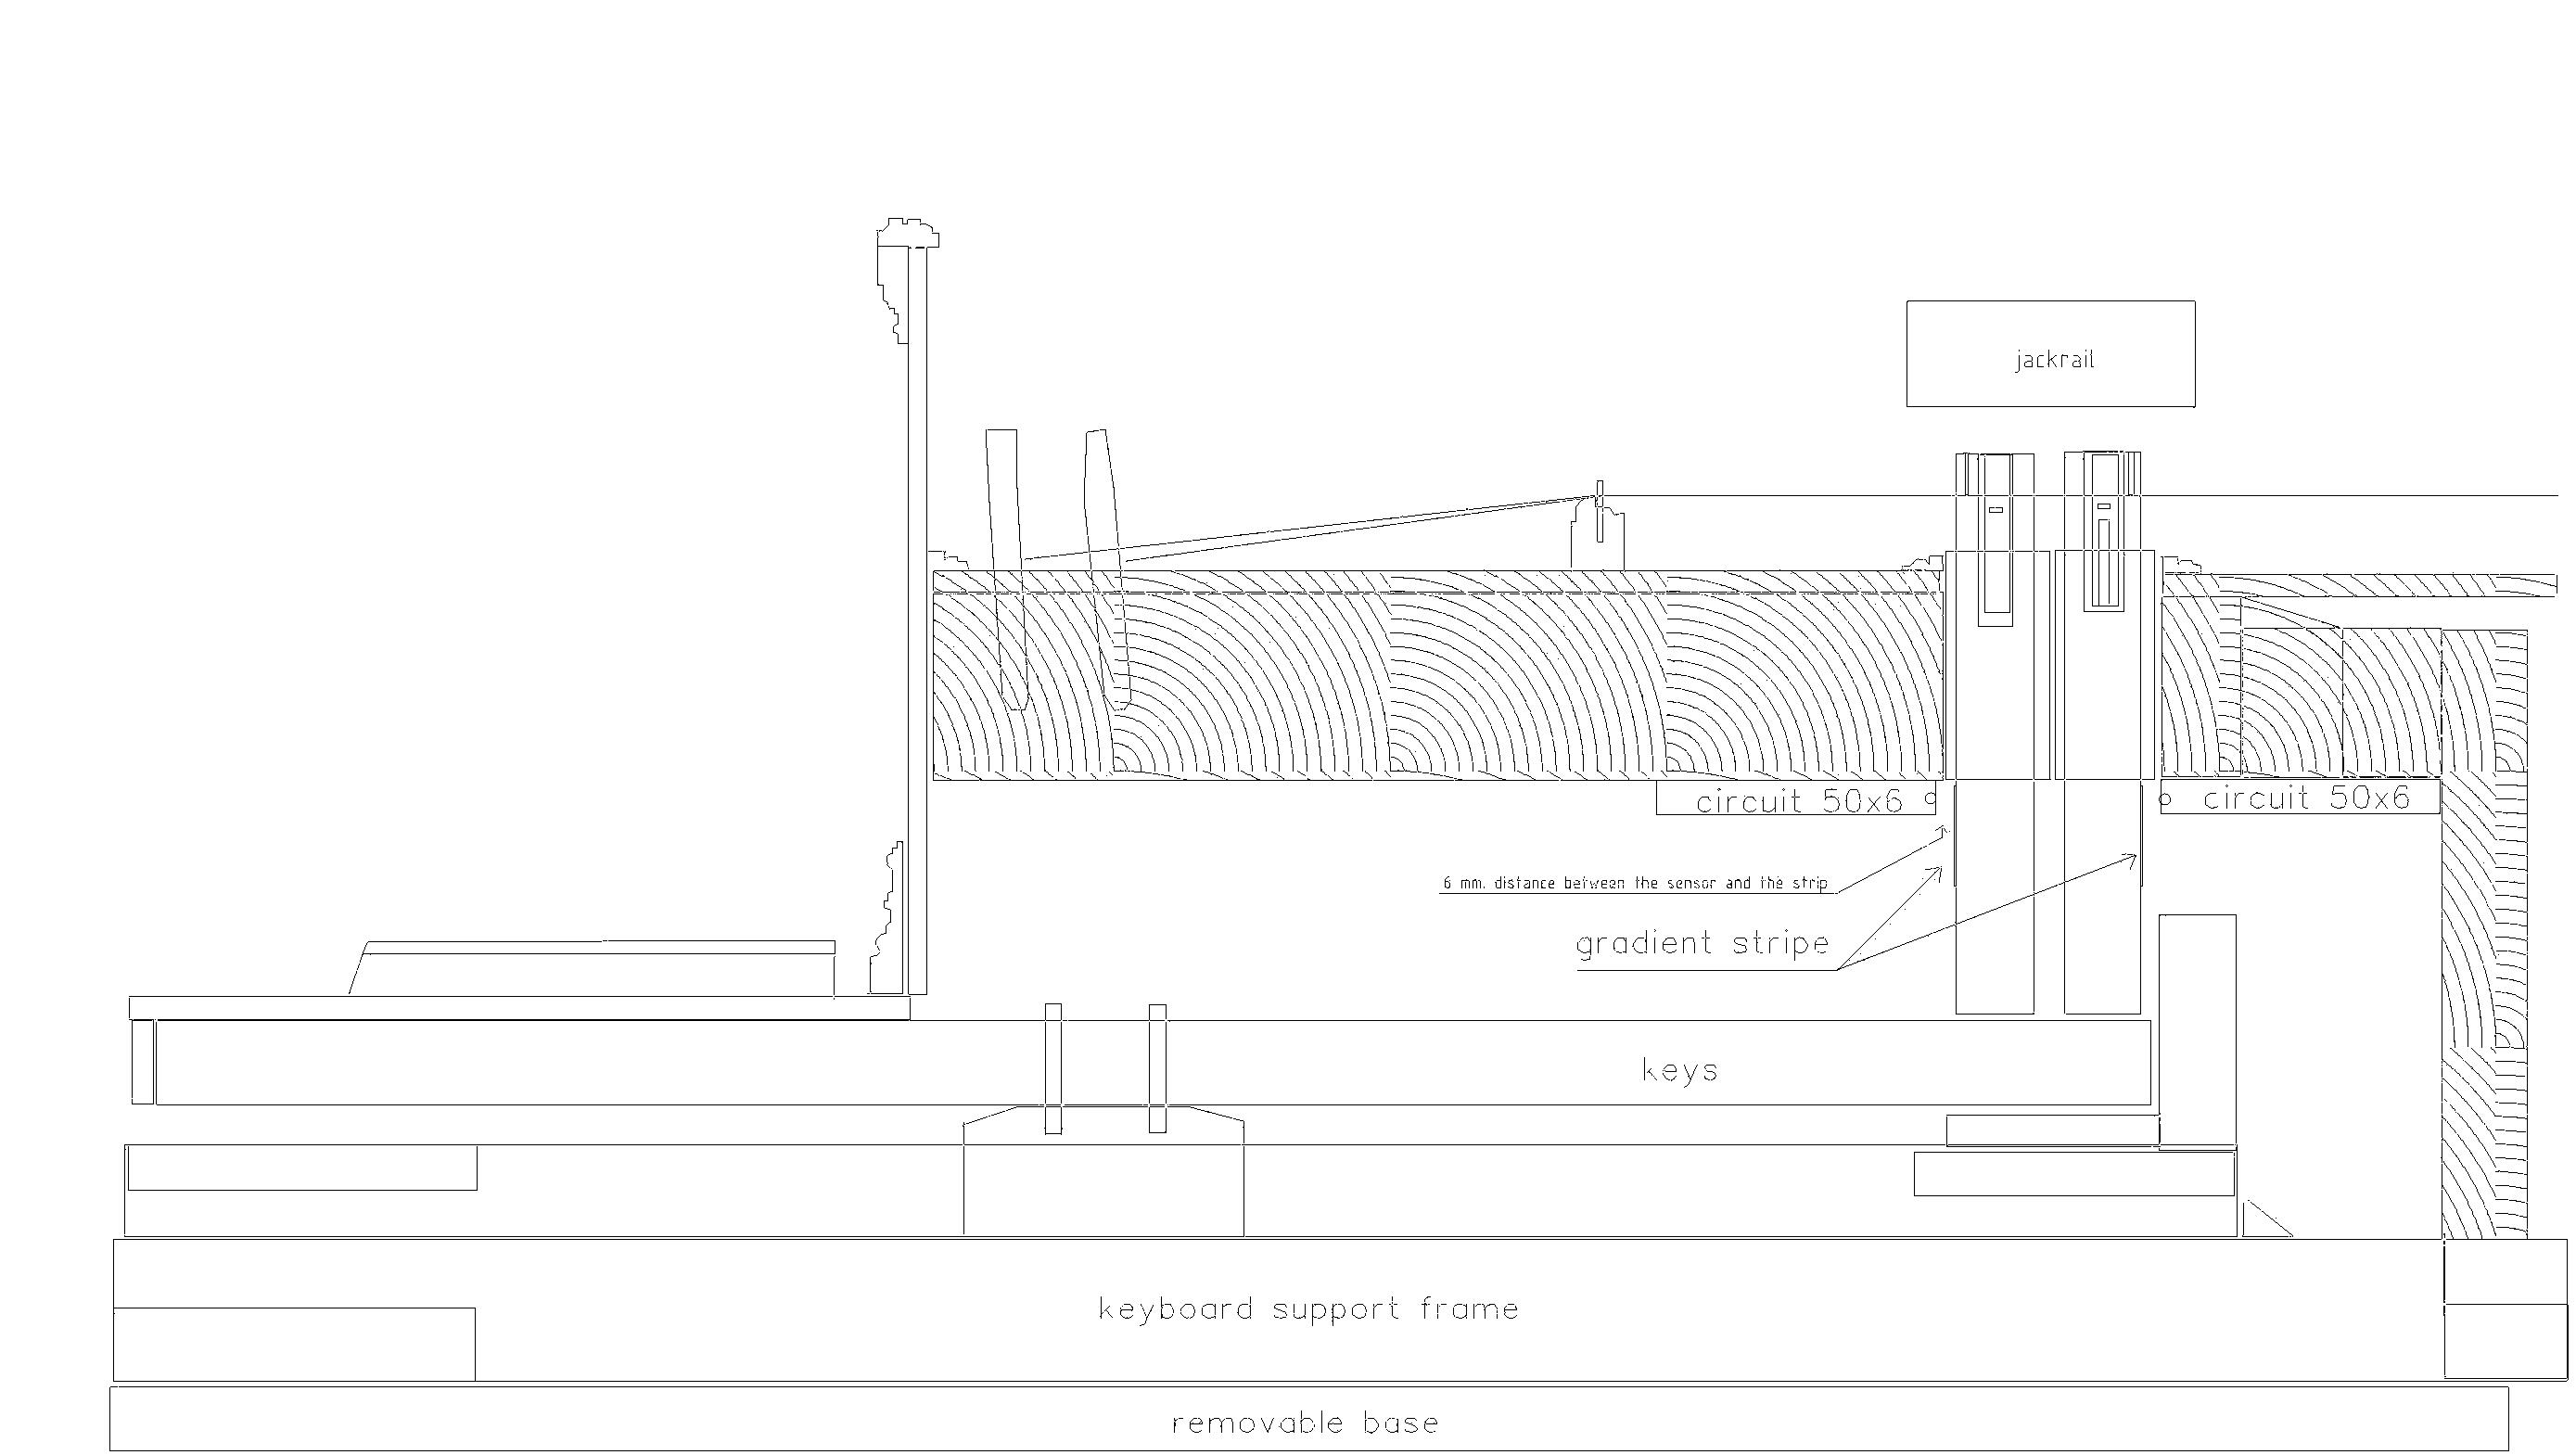
\includegraphics[width=\linewidth]{src/images/CrossSectionSensorPlacement.jpg}
%     \caption{Cross-section illustrating sensor placement relative to the jack mechanism.}
%     \label{fig:cross-section}
% \end{figure}

\begin{figure}
    \centering
    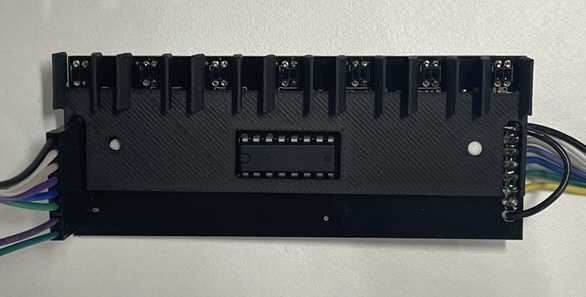
\includegraphics[width=\linewidth]{src/images/sensor-board-w-baffles.jpeg}
    \\
    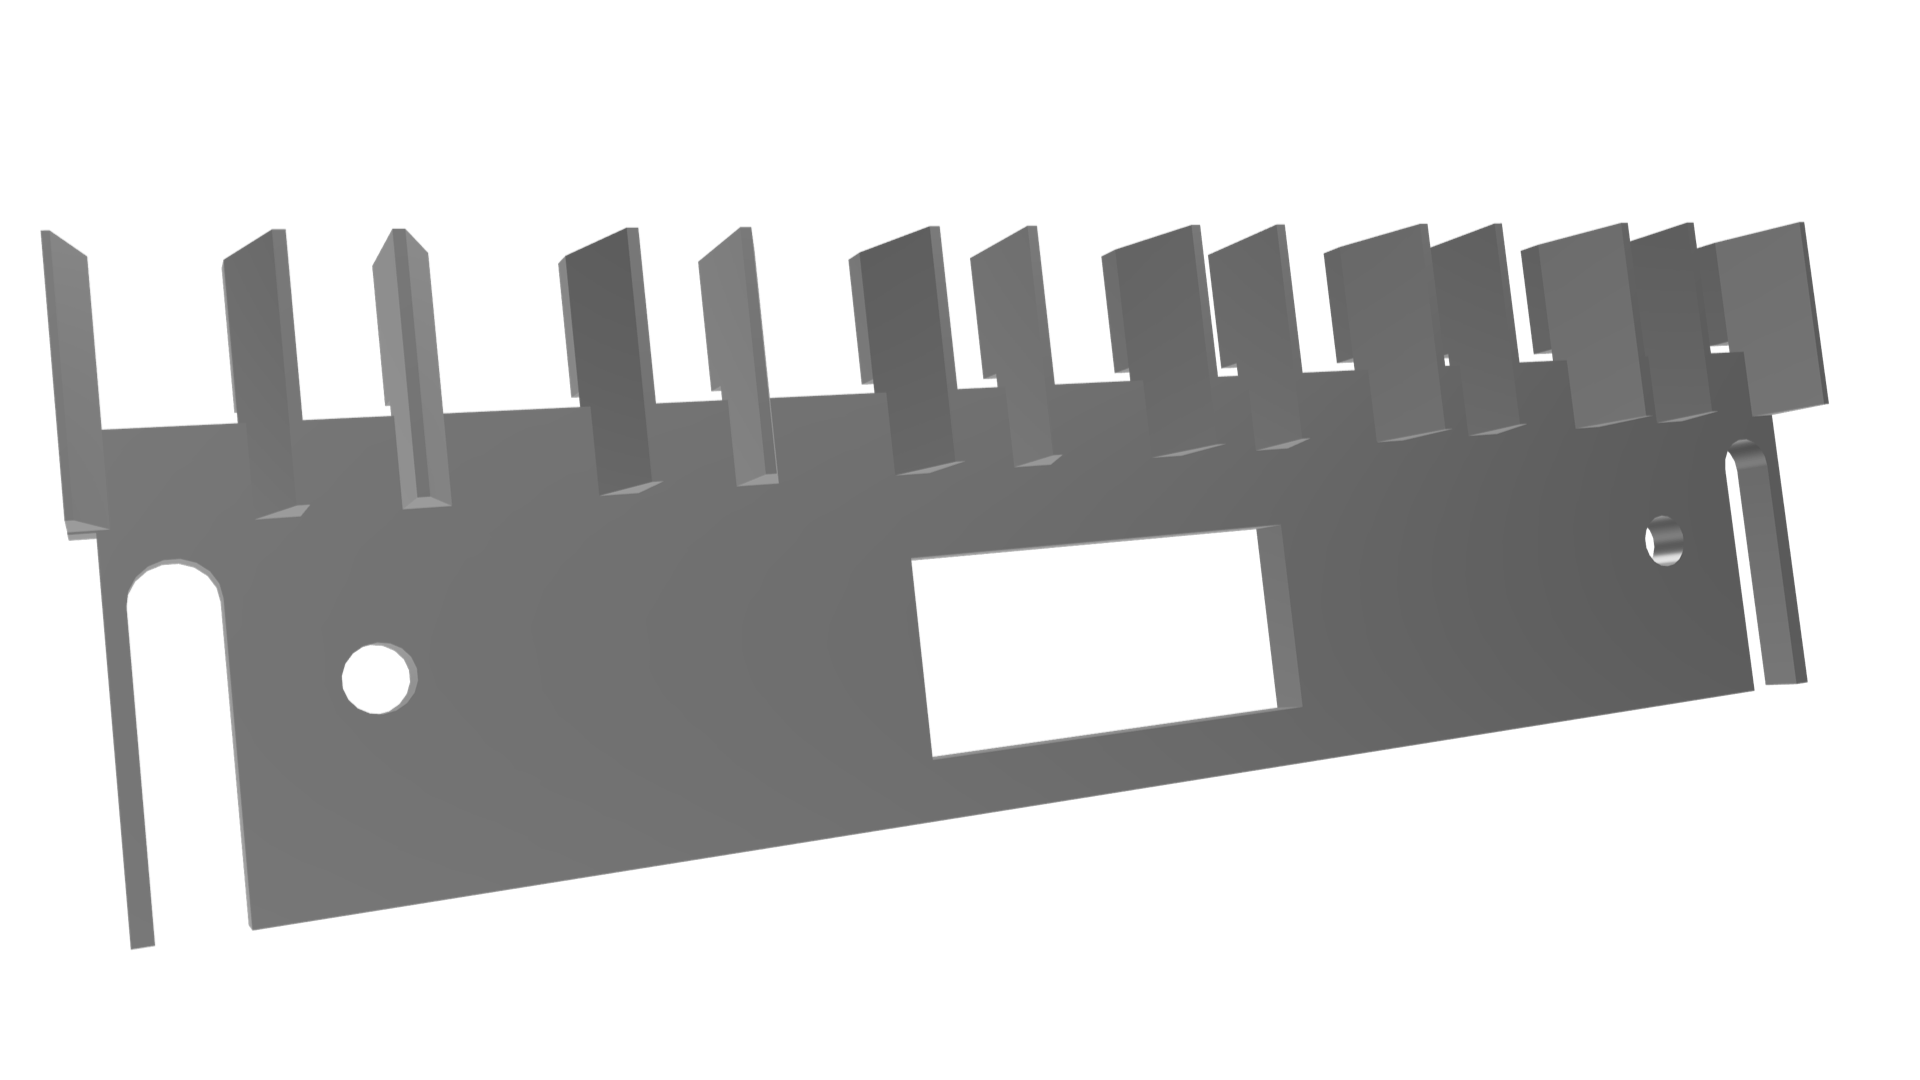
\includegraphics[width=\linewidth]{src/images/baffles.png}
    \caption{Baffles designed to prevent cross-talk between adjacent sensors.}
    \label{fig:baffles}
\end{figure}

\begin{figure}
    \centering
    \includegraphics[width=\linewidth]{src/images/serial_monitor.png}
    \caption{Arduino IDE serial plotter used for calibration of sensor thresholds. \texttt{M} and \texttt{m} represent the maximum an minimum value of digitised data. \texttt{K} and \texttt{T} are the values of the sensor and threshold being calibrated, followed by a two digit number denoting the sensor index (in this case sensor 32).}
    \label{fig:serial_monitor}
\end{figure}

% \section{Hardware Design}

% For the first iteration the data from the sensor would simply be used to test when a threshold had been passed. On passing the threshold, a message will be sent to trigger the playback of a corresponding note.

% For the initial prototyping stage, modifying an existing harpsichord was considered though ultimately discarded. An existing instrument would
% have provided a test for scaling the electronics, but internal measurements and layout would have been too different. 

% Using a similar approach to Timmermans' Haptic Key project, \cite{Timmermans2020}, our first step was to fabricate or procure a model of a single working key. San Colombano provided a model 3-key of a harpsichord mechanism by Graziano Bandini (Figure \ref{fig:3key}).

% \subsection{Sensor Criteria}\label{sensor-criteria}

% A set of criteria was drawn to which the final sensor system would have to satisfy. These criteria were used to evaluate the feasibility throughout the prototyping phase.

% \begin{itemize}
% \item
%   Non-invasive: The sensor system should not require major modifications
%   to the interface on which it is installed.
% \item
%   Low Latency: Reading sensors and then triggering an output should have
%   a low latency. Following \cite{Jack2016} an latency was set as 10 ms
%   with an upper limit set to 25 ms beyond which the sensors would be
%   deemed unusable
% \item
%   Reliable: Data obtained should be reliable and accurate enough not to
%   result in false positives or false negatives without extensive
%   filtering
% \item
%   Scalable: The system should be scalable both economically and
%   temporally. Given the open source nature of the project, it could not
%   be prohibitively expensive to carry out. Also any system that would
%   work on a single key would have to scale financially to potentially 50
%   or more. The time required to install and calibrate the sensors would
%   also have to scale.
% \item
%   Expandable: Any sensor system should be functionally expandable to
%   allow for the usage of the data for control over other parameters.
% \end{itemize}



% The sensor system was designed so that they would not require any equipment outside what can commonly be found in a maker space at a university for assembly. This decision was motivated by the project's goal to be open source and reasonably recreated without procuring additional specialist equipment.


% The electronics system can be divided into two designs, the "sensor board" (Figure \ref{fig:7-sensor-board}) for components for detecting jack displacement and controller board for collecting and processing sensor signals.

% \begin{figure}  
%   \centering
%   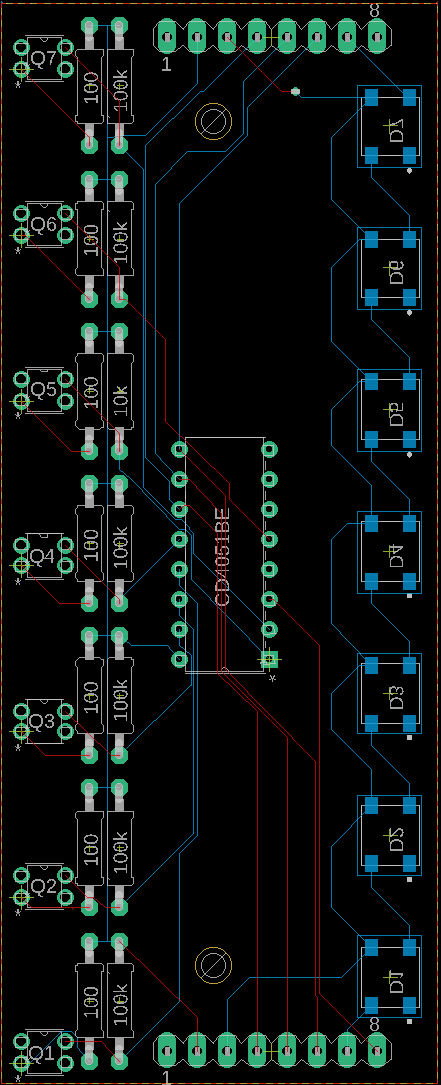
\includegraphics[angle=-90,width=\linewidth]{src/images/7-sensor-board-v0.1.0.png} 
%   \caption{} 
%   \Description{} 
%   \label{fig:7-sensor-board}
% \end{figure}

% \subsection{Sensor board}\label{sensor-board}

% The 49 optical sensors are divided across 7 PCBs each containing

% \begin{itemize}
% \item
%   x7 QRE1113 optical sensors
% \item
%   x7 100 $\Omega$ resistors
% \item
%   x7 10 k$\Omega$ resistors \footnote{a update on the design showed these could be reduced to a single resistor.}
% \item
%   x1 CD4051BE Multipexer
% \end{itemize}

% A number of sensors were tried before the final system was decided upon. 
% Sensors tested for the design included, a 6-degrees-of-freedom inertial measurement unit, reed and hall sensors paired with magnets, and light-dependant resistors mounted to the jack rail.
% None of the above satisfied the sensor criteria described and were thus discounted.

% Following from the work in \cite{McPherson2013, McPherson2019}, we tested
% a system using the Fairchild QRE1113 \footnote{Fairchild, now ON Semiconductor, QRE1113 datasheet \url{https://www.onsemi.com/download/data-sheet/pdf/qre1113-d.pdf}}. The
% QRE1113 is a combination infrared LED and phototransistor sensitive to
% IR light. The phototransistor of QRE1113 provides data on how much light
% is present and in particular how much light is being reflected from a
% surface. Since reflected light will be proportional to the distance of
% a surface it is a good, close-proximity, distance sensor. Distance is
% the way in which the instruments in \cite{McPherson2013, McPherson2019}
% function as well the Moog Piano Bar from which it took inspiration.

% The limitation for taking a distance approach is that there is not one
% but 2 jacks per key. For each jack to be measured independently the data
% would need to come from the jacks themselves.

% % They \emph{could} be used and individual trigger points set in
% % calibration, but this creates new problems.

% \begin{figure}  
%   \centering
%   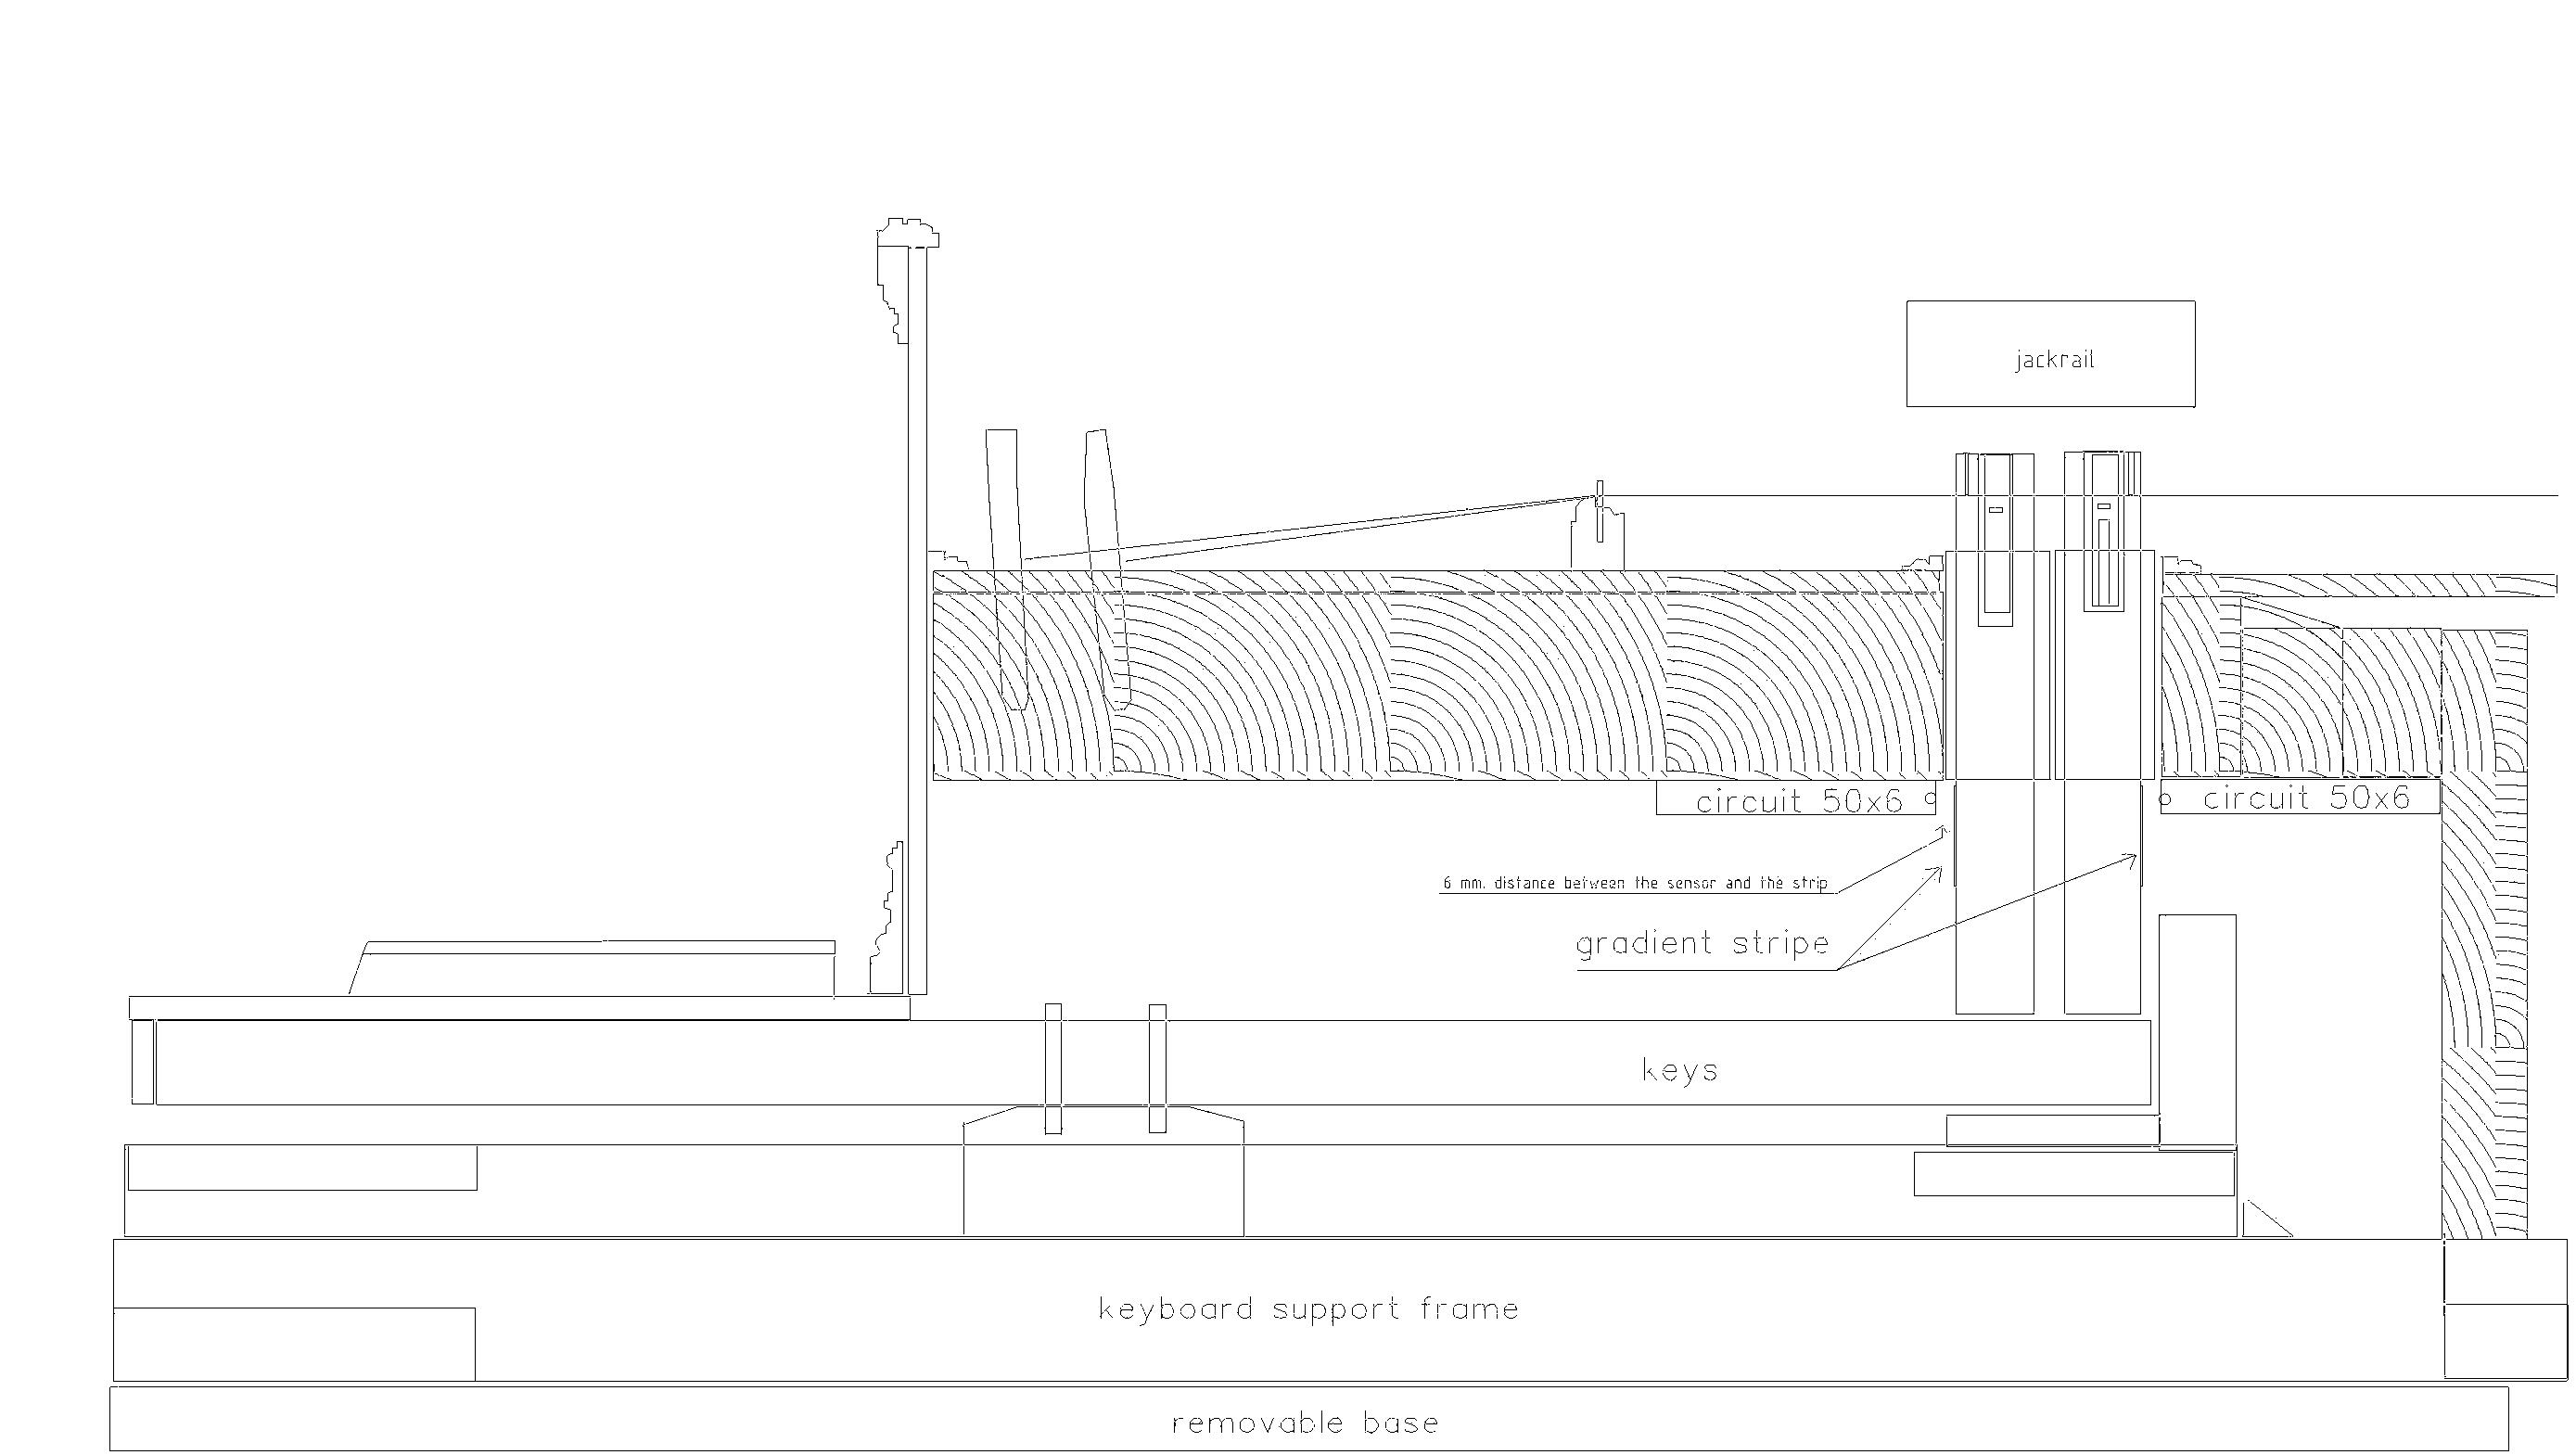
\includegraphics[,width=\linewidth]{src/images/CrossSectionSensorPlacement.jpg} 
%   \caption{} 
%   \Description{} 
%   \label{fig:cross-section}
% \end{figure}



% The optical sensors were directed at a greyscale gradient printed on a sticker and applied to the side of the jack.
% This was first trialled using a generic inkjet printer and double-sided tape. 
% For the final iteration, the stickers were printed on Coala 1D 100 Gloss PG 100 $\mu$m white gloss monomeric PVC with permanent grey acrylic dispersion adhesive \footnote{Datasheet: \url{https://www.antalis.co.uk/mediashare/g4media/pdf/TS_EN_COALA_1D_100_GLOSS_P_00_ISS_15022023.pdf}} using a HP Latex 115 and then cut with a Summa 150 roll cutter. 
% The printer and roll cutter greatly reduced the manual labour for cutting stickers meaning the process would scale from the 6 jacks of the 3-key to the 98 jacks of the 49-key model.

% \begin{figure}  
%   \centering
%   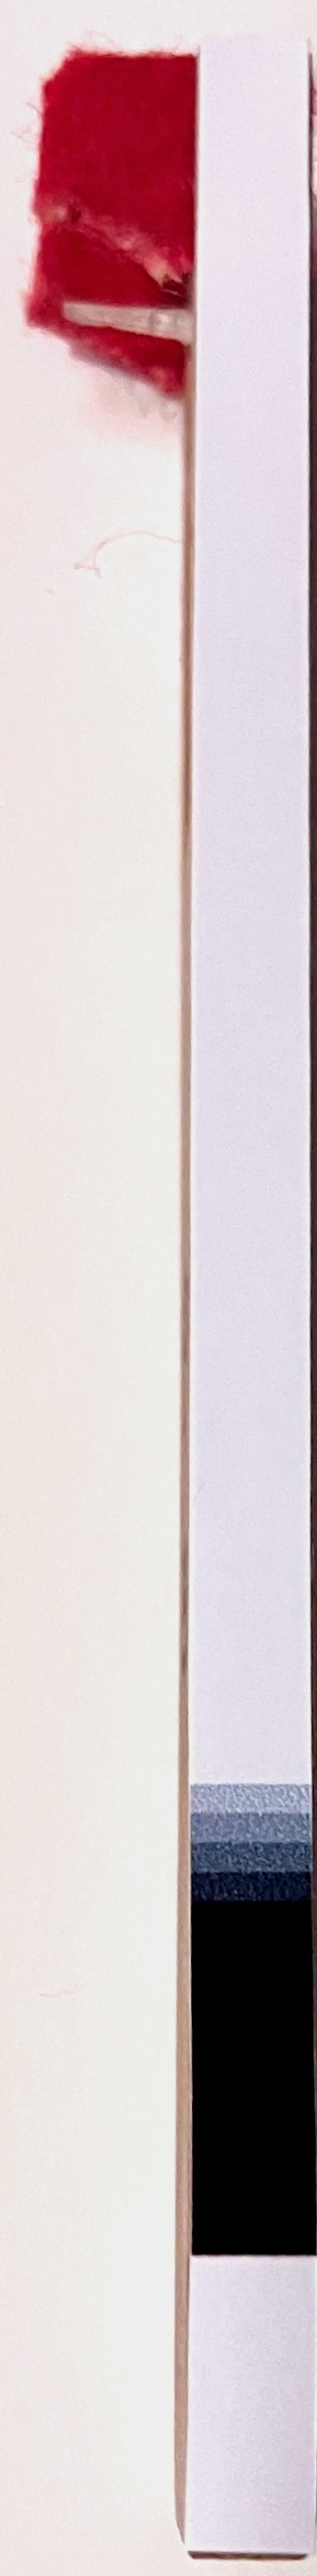
\includegraphics[angle=90,width=\linewidth]{src/images/jack-w-tag.jpeg} 
%   \caption{} 
%   \Description{} 
%   \label{fig:jack-w-tag}
% \end{figure}

% During testing it was found that their was a considerable amount cross-talk between adjacent sensors. 
% This meant the reading from key would be affected by the movement of the key next to it. 
% The cross-talk was assumed to be as a result of light reflecting from other jacks.
% Given that IR is used this was difficult to confirm by sight. 
% A set of baffles was designed for the PCB that would wrap round the jack and stop light from other jacks or sensors \ref{fig:baffles}. 
% The baffles were printed on a BAMBU X1 3D printers using PLA plastic. A dark pigmented PLA was used to avoid IR light simply being diffused. 
% After the baffles were fitted, the cross-talk was eliminated.

% \begin{figure}  
%   \centering
%   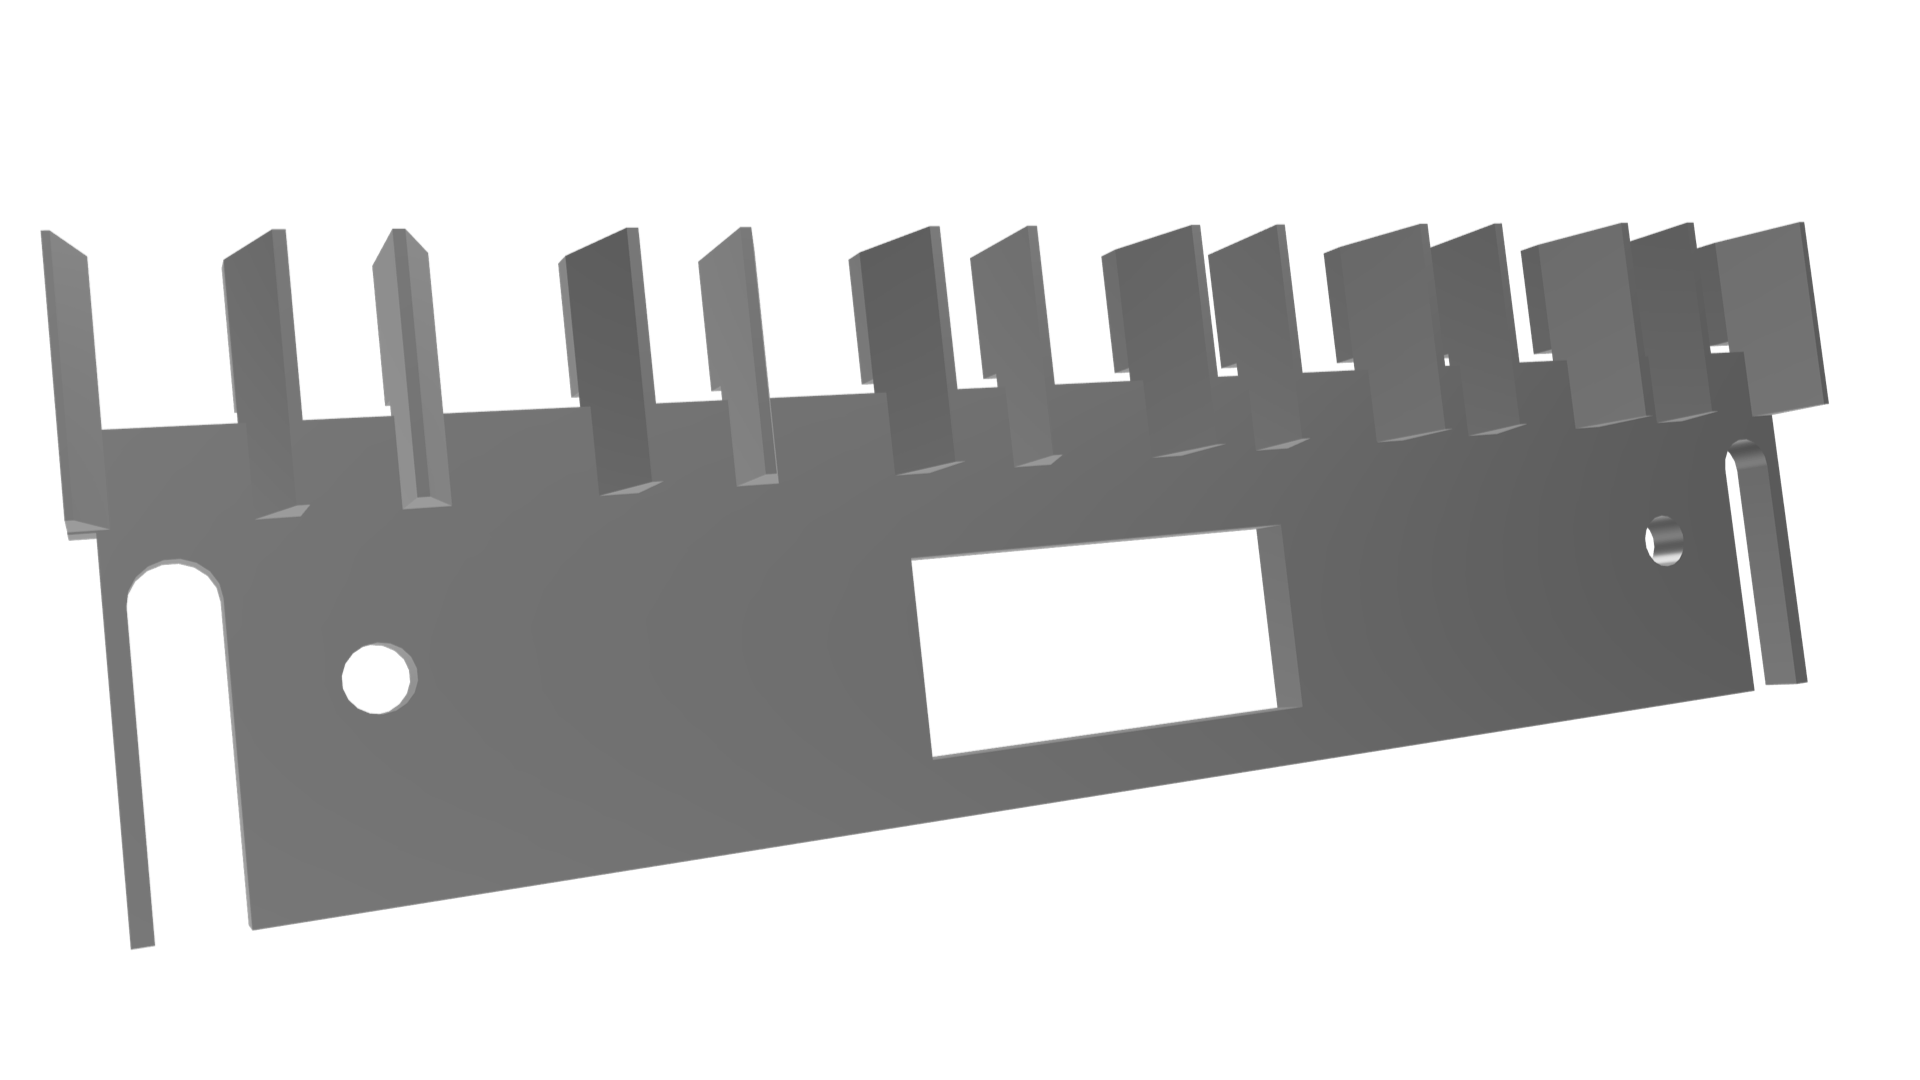
\includegraphics[,width=\linewidth]{src/images/baffles.png} 
%   \caption{} 
%   \Description{} 
%   \label{fig:baffles}
% \end{figure}



% Calibration to pluck thresholds were to be carried out manually.  To allow for easy identification of the sensor being addressed during the calibration process, RGB LEDs were integrated into the design. The LEDs were also used in the identification of any malfunctioning or un-calibrated sensor.



% TLC5940 or other PWM driver such as in \cite{McPherson2013} add robustness should an LED fail, but complexity to assembly process. 
% Instead, the design uses addressable LEDs with integrated driver that share the same data line. 
% This has the limitation where a faulty LED will stop all subsequent LEDs in the line from working. 


% The BLE Nano has 8 ADC pins connected to one ADC channel via a multiplexer. 
% We avoided the complexity of communicating multiple microcontrollers and instead used a Texas Instruments CD4051B multiplexer on each sensor board.
% An 8-channel multiplexer was chosen as the model has 49-keys and a division of 7 PCBs each containing 7 sensors.
% The multiplexer reduced the 7 sensor signals to a single channel. The CD4051B is addressed with a 3-bit which necessitates 3 digital channels.
% Transistor / Op-amp circuit could have been used similar to the one in \cite{McPherson2013}. 

% \subsection{Controller Board}\label{controller-board}

% Controller board designed around Arduino nano form factor. The Nano is
% connected through headers to allow easy switching between chips. Should
% another chip in a Nano for factor be found it could supplant the current
% Nano without any need for a redesign.

% The first version of the board exclusively used 2.54 mm pitch headers.
% The reasons for this were flexibility when creating cable looms and to
% leave open the possibility of rewiring the PCB.

% This was the case for the LEDs as they initially were to be powered on
% 5V. It was discovered that the 3V regulator of the nano was sufficient
% to power all LEDs at a lower brightness while reducing current draw.
% Since brightness was not important.

% The 2.54 mm pitch headers had two major drawbacks. First, the orientation
% of the cables could be reversed, which in the best case scenario would
% simply mean the system did not work correctly and in the worst case it
% could potentially damage the components.

% Secondly, the headers do not connect securely and wait of the cabling
% was enough for components to become disconnected as the harpsichord was
% handled.

% To address this, once the wiring for the controller board was finalised
% a new design was drafted this time using JST-PH connectors. No
% commercial cables were immediately available in the configuration and
% length required, as such a cable loom needed to be made which meant
% crimping cables by hand. A crimping tool from JST is prohibitively
% expensive compared to the cost of other components in the project
% \footnote{from RS \url{https://uk.rs-online.com/web/p/crimp-tools/6880877}
% £508 (inc. VAT)}. The crimping tool also appeared to be uncommon and was
% not readily available in the workshops at the project's disposal.
% Eventually a tool was found, but an alternative approach was also
% researched in order to maintain the criteria of accessibility.

% A locator was adapted from a creative commons STL model \footnote{\url{https://www.thingiverse.com/thing:1646016}} that allowed a generic crimping tool to be adapted for use with JST-PH crimps. 

% \subsubsection{Arduino Nano BLE}\label{arduino-nano-ble}

% Arduino Nano BLE was chosen for a few reasons. The Nano form factor was
% appealing as it would allow for easy changes between chipsets without
% requiring any rewiring and thus no new PCBs would need to be created if
% a better alternative was found later in the project. Another benefit to
% the Arduino Nano boards was that typically had native-USB meaning the
% could be programmed as a hardware USB MIDI device directly.

% The Nano BLE was used in the initial stages for its integrated inertial measurment unit.

% When it was finalised that the project would proceed using the QRE1113 a
% number of microcontroller units (MCU) were considered.

% The MCUs considered were the Arduino Nano 33 IoT, Arduino Nano 33 BLE,
% Arduino Nano ESP32 and STM32 NUCLEO-L031K6.

% A rough performance test was later carried out using an STM32
% NUCLEO-L031K6, a Nano ESP32 and the BLE. The Nano BLE was found to be
% more performative. To execute a single sensor read cycle of the firmware
% the STM32 took 40 ms, and both the Nano ESP32 and Nano BLE required 11 ms
% on average. The Nano ESP32 had high variability so it was decided to
% continue with the Nano BLE. 



% BLE functionality also meant if the cable connection between the nano
% and computer running audio synthesis was impractical, BLE MIDI was
% available as a fallback. The Nano BLE also has a 12-bit DAC, which
% provided a contingency should the default 10-bit not be sensitive enough
% for the signal from the sensors.

% Initially a Nano IoT was used for both WiFi and Bluetooth Low Energy
% functionality, but it was found that 2 ADC channels were in fact not
% useable and would have required additional multiplexers.

% \subsubsection{EEPROM / NVRAM / FRAM}\label{eeprom-nvram-fram}

% There would need to be the ability to store values on non-volatile
% memory so that the electronics could be powered-down without losing
% data.

% Adjusting the values through firmware would not have been flexible or
% practical. Instead an Ferroelectric RAM unit was chosen and connected
% using an SPI interface. NVRAM or EEPROM would have sufficed and the FRAM
% was primarily chosen for it's ready availability.

% Most microcontrollers have some variety of non-volatile program memory
% that can be read and writ accessed but in most cases this memory is
% cleared during compilation and re-flashing. The small cost was far
% outweighed by the potential for data loss if using onboard RAM.



% SD card would provide an easier way to interact with calibration data.
% The position of the controller board did not permit easy access.
% Reliability and speed was preferred over storage capacity.



% \subsection{Power}\label{power}

% All electronics combined draw around 1.1 A of current at 5V with some fluctuation during start-up.

% Arduino BLE has some functionality disabled to limit current draw.

% Ideally the unit could be bus powered from USB.

% The sensors are in a state of constantly drawing power. 
% It is possible that powering only when data is required could be reduce power enough.

% Current designs have a separate MIDI device for each jack row. 
% Combining the devices and also reducing current draw to below the common 0.5 amps for a USB port would certainly be a challenge.

% \section{Firmware Design}\label{firmware-design}

% Arduino platform chosen for wide adoption, relative ease of use and
% library support for components.

% Firmware checks components are connected then reads the FRAM to see if
% threshold data is already present. The rotary encoder and it's momentary
% switch are polled for any change in state. A key is selected with the
% rotary encoder while the momentary switch is used for changing between
% states for key selection and threshold adjustment A double click of the
% rotary encoder writes the current threshold values to FRAM. The sensors
% for the current multiplexer channels are polled. If any sensor reads
% above the threshold when it was previously below a MIDI On message is
% sent. For the reverse case where the value was below the threshold when
% it was previously above, a MIDI Note Off message is sent.


% \section{Implementation}\label{implementation}

% \begin{figure}  
%   \centering
%   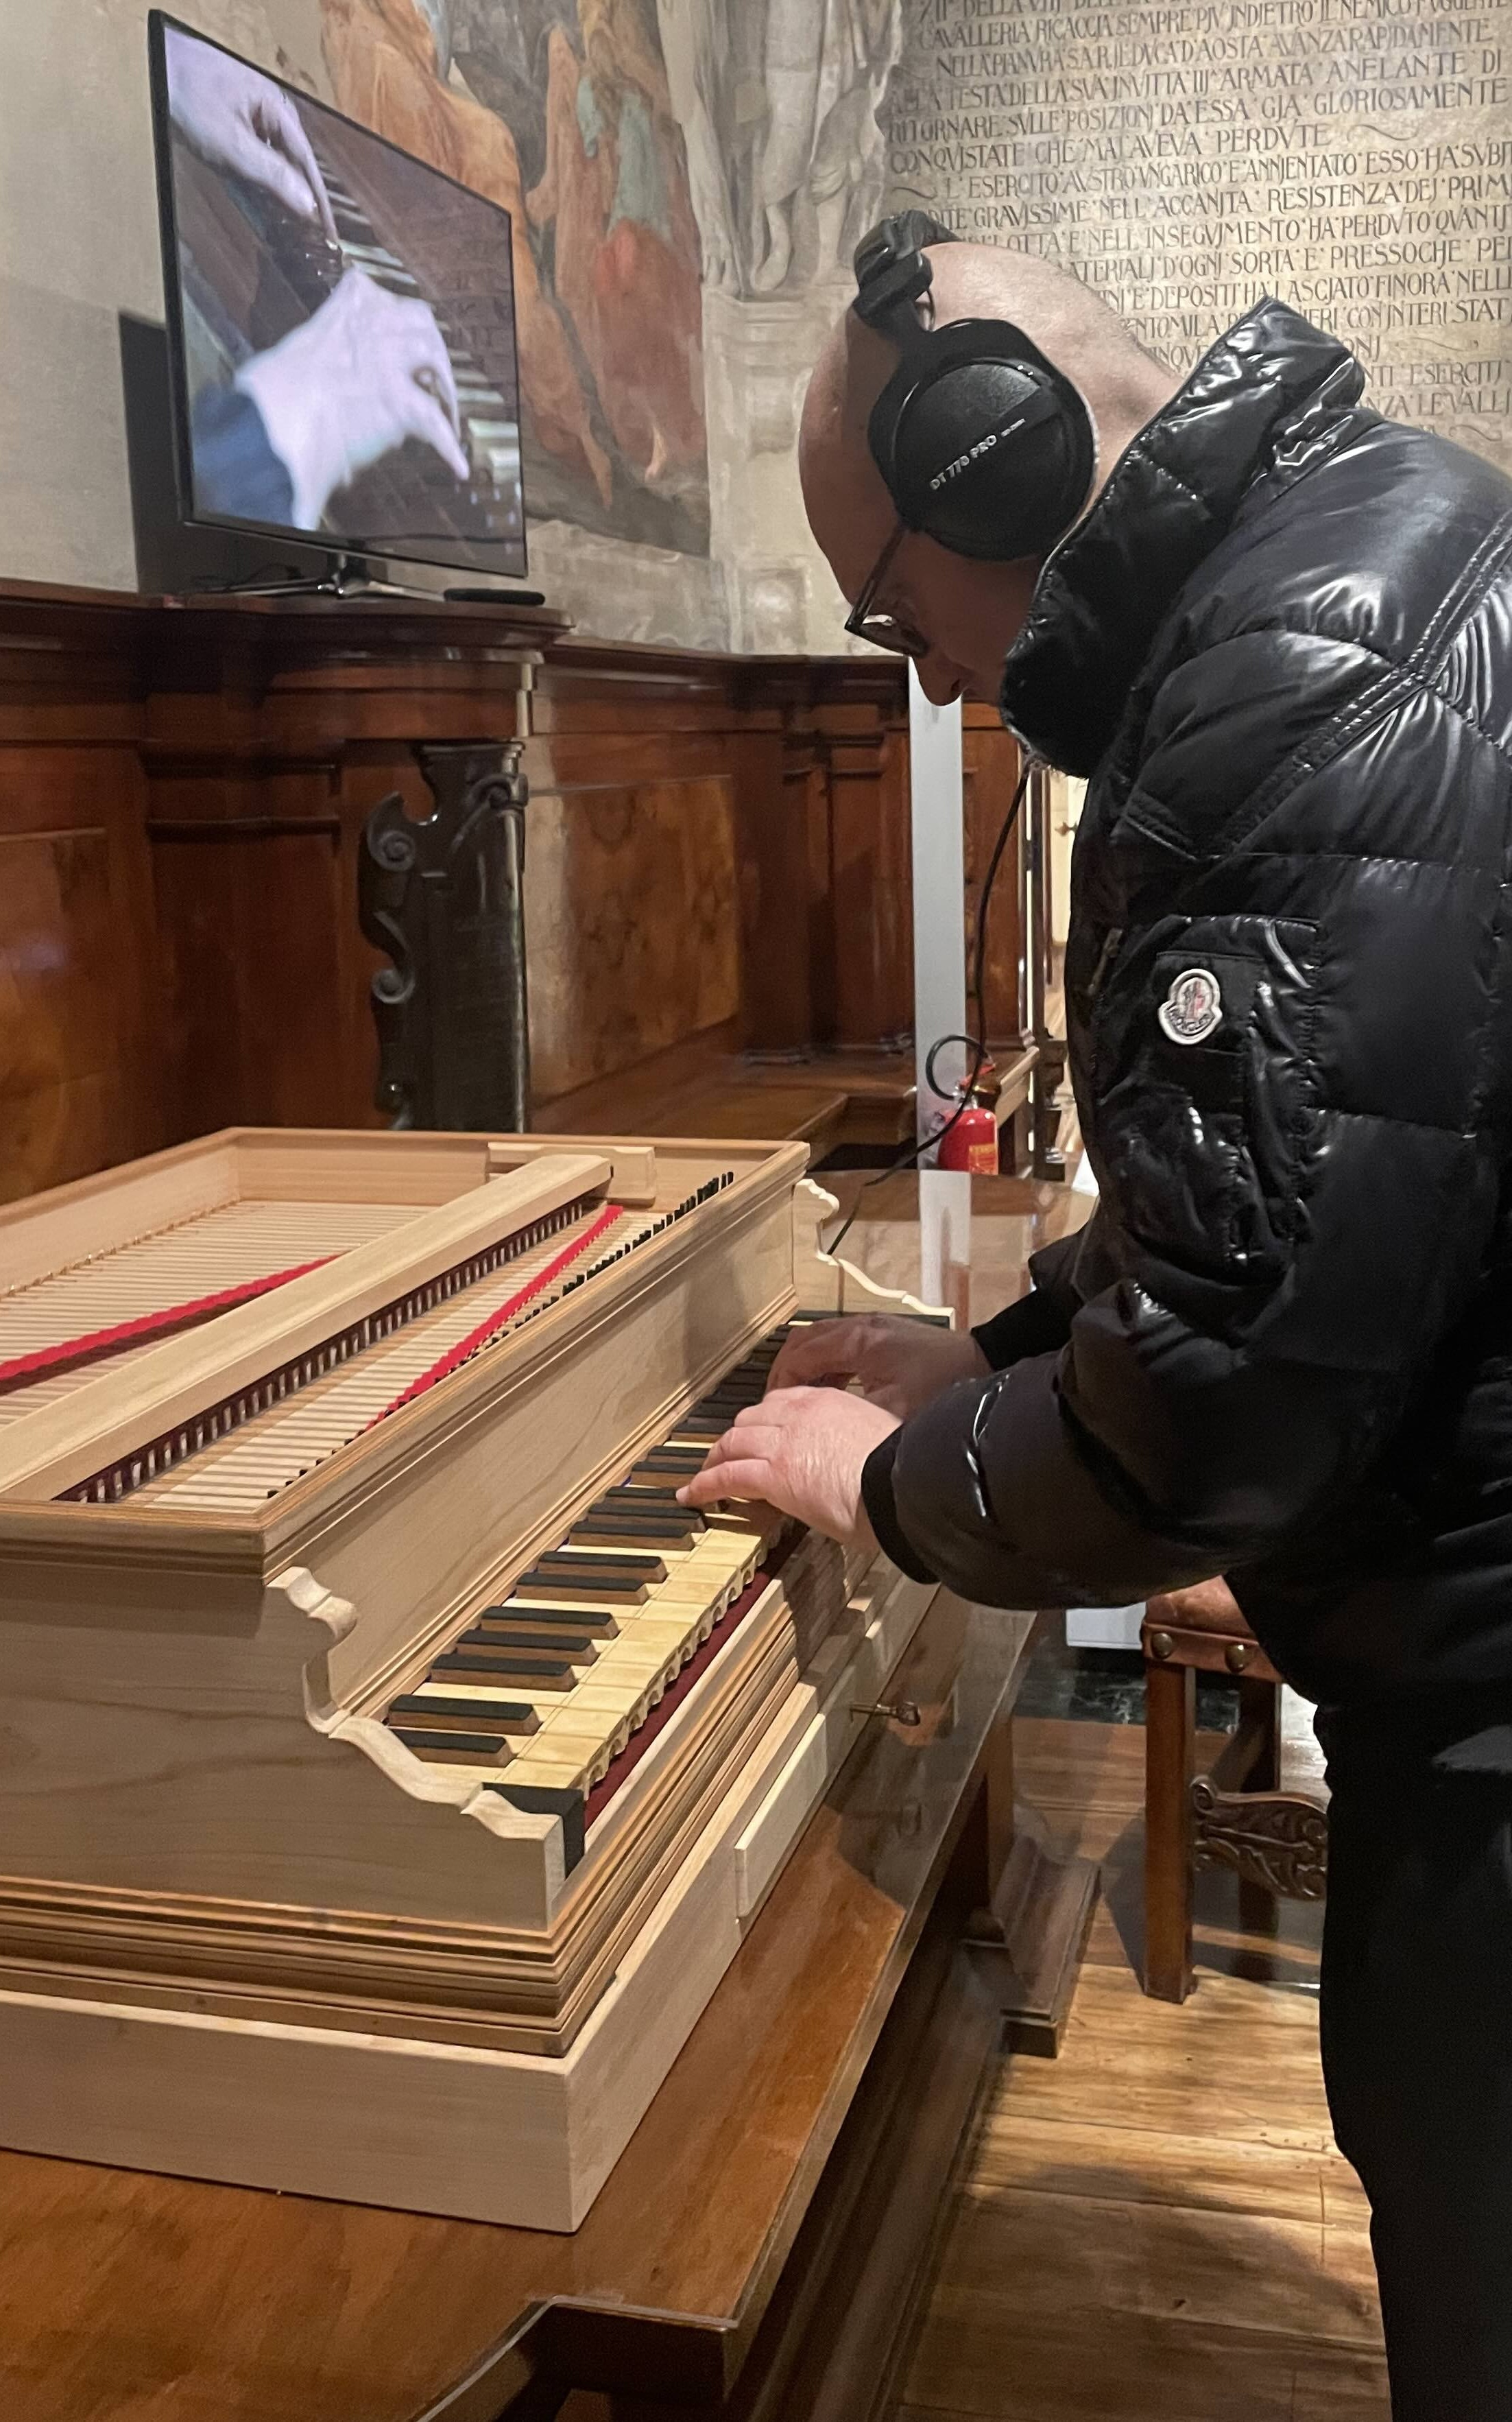
\includegraphics[,width=\linewidth]{src/images/exhibition-user-1.jpeg} 
%   \caption{} 
%   \Description{} 
%   \label{fig:exhibition}
% \end{figure}

% \subsection{Installation}\label{installation}

% The electronic components were partly pre-assembled at the university of
% Edinburgh. Though all measurements were known ahead, enough flexibility
% was needed to allow for problems to solved in situ.

% The final assembly took place at the NEMUS lab at the University of
% Bologna over the final week in October 2024 for delivery at San
% Colombano for exhibition in the first week of November in 2024.

% A misreading in the original clearance between the keys and the PCB
% meant that the keys were blocked entirely from moving. A 10 mm by 15 mm
% section was milled out of each key to create extra
% clearance. The milling required the removal, shortening and refitting of
% the leather pads for the jacks. The extra work
% added an extra day to the full install.

% \begin{figure}  
%   \centering
%   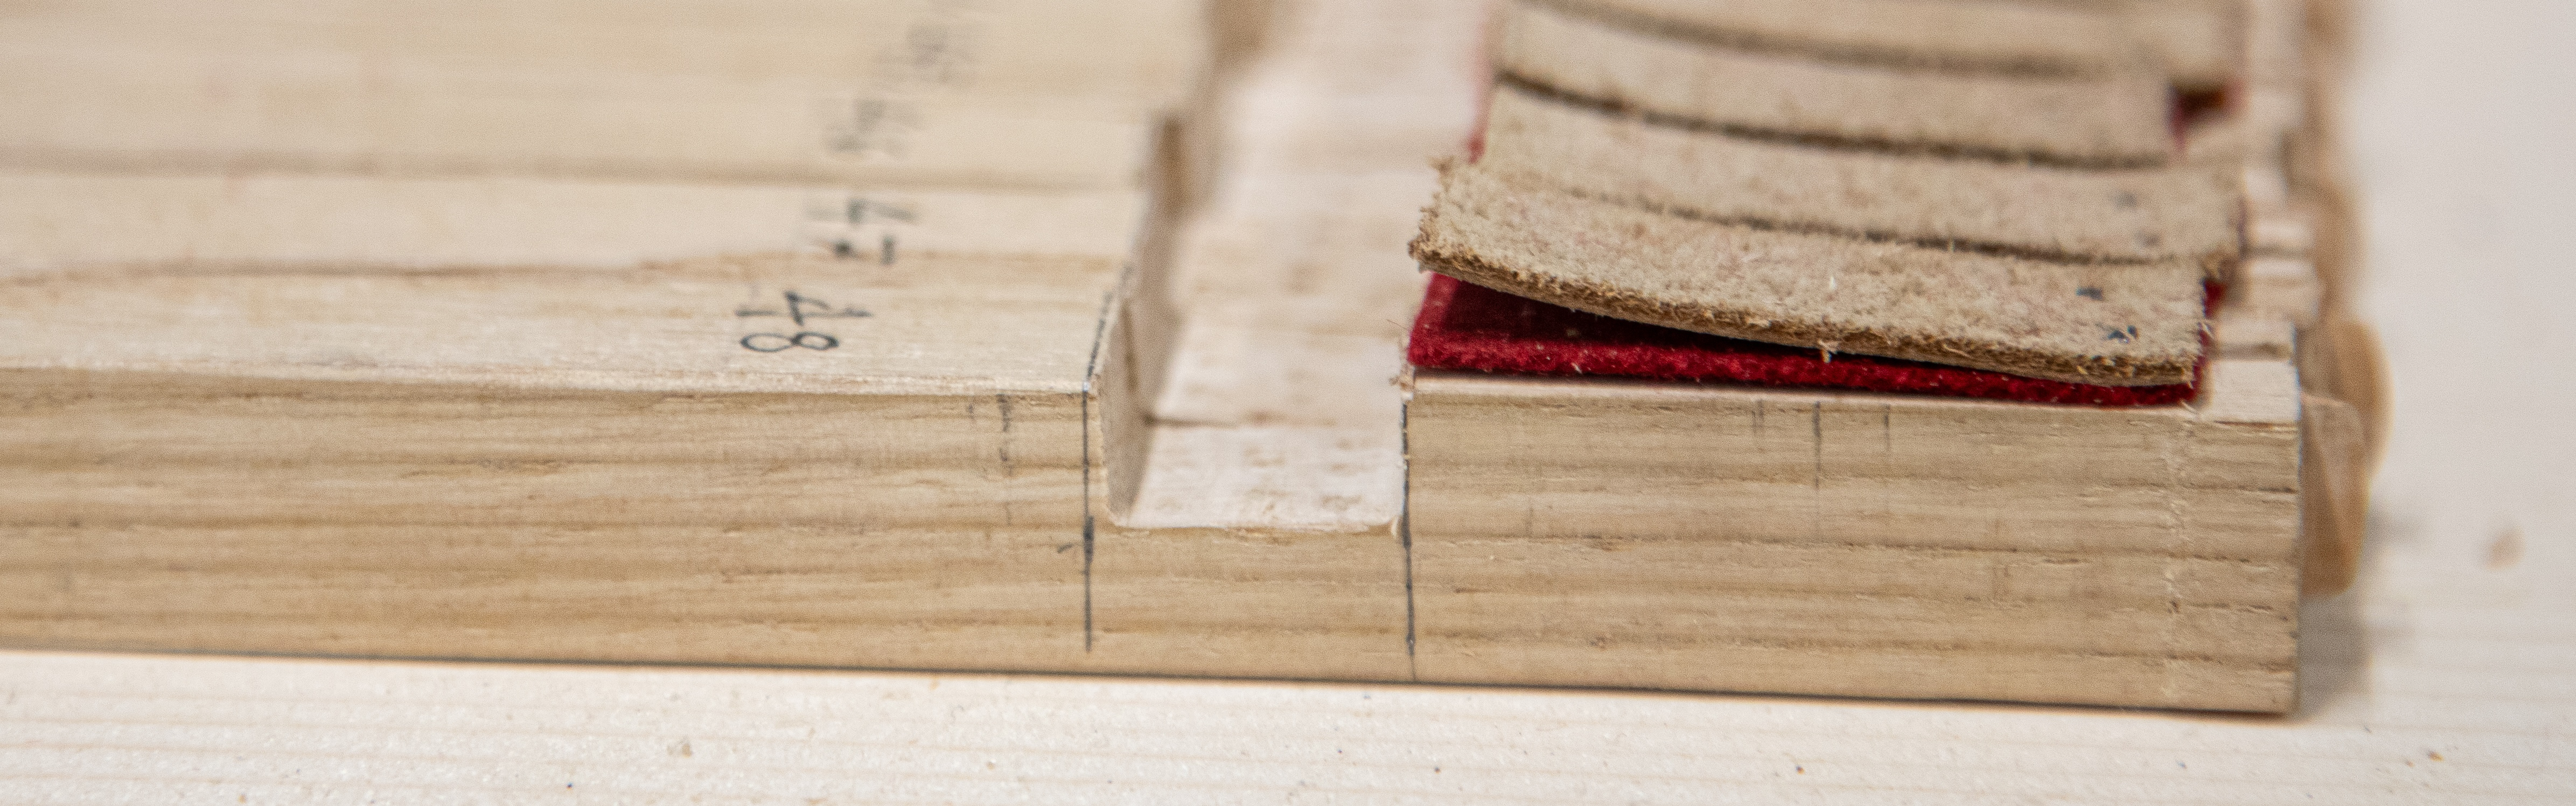
\includegraphics[width=\linewidth]{src/images/milled-keys.jpg} 
%   \caption{} 
%   \Description{} 
%   \label{fig:milling}
% \end{figure}

% A redesign of the PCBs meant that removing the material would no longer
% be necessary.

% The PCBs shared power and data lines for components with the exception
% of the output from the multiplexer. Ribbon cable was cut to size to
% allow for some room to readjust the distance of the sensors from the
% jacks. The data signals from each PCB were connected using a separate
% cable loom. Soldering cables and inspecting each join required another
% day work. This did allow for readjustments to the position of the
% controller board Measurements of the rear chamber did not match with the
% Mac Mini that was to be used a different layout was decided for fitting
% the controller board/ Cutting cables to size allowed for a great deal of
% flexibility but at the cost of time. After the first install it was
% clearer what constraints were in place for fitting and an alternative
% wiring system using flat flex cable was implement (discussed in
% \textbackslash section)

% Fitting PCBs required the removal of all keys. The support brackets were
% assembled and screwed into the the underside. With the harpsichord on
% it's back the sensors were tested to ensure an expected range.
% Self-tapping round head screws were used to to attach the brackets. The
% screws were not over tightened to allow for brackets to move. The
% brackets were not easily adjusted once the key were replaced. Adjusted
% to a best average with subsequent adjustment carried out on the
% microcontroller.

% As the PCBs were fitted the jacks had the gradient stickers applied to
% them. The jacks had been coated with a varnish on the short side to
% provide a better surface for the stickers to adhere to. After the
% stickers were applied excess material was trimmed from each jack. The
% jack were then check that they moved freely in their slot.

% After fitting the PCBs preliminary calibration was carried out. Before
% the keys were refitted the jacks were put back in place. The data from
% each key was confirmed to be in a similar range. Any key showing
% anomalous data had it's jack removed and re-inspected. The PCB fitting
% process and refitting required another day as faults were found in
% wiring or misalignment of the stickers. After the sensors were
% confirmed to be functioning the keys were put back.

% The calibration workflow was with \anon{Dr. Craig Webb} who was unfamiliar with
% the system. Adjustments were made to the firmware to to make it more
% intuitive for the user. Addressable LEDs became vital as it allowed for
% easy identification of the key being calibrated. They were also used to
% identify any keys whose current reading was beyond what was expected.

% The rotary encoder was used as the interface to select a key, adjust
% it's threshold and update the Ferroelectric RAM (FRAM) with new values.

% A process was implemented where the key was selected by playing, but
% this caused problems in situations where the data was unusual due to
% misalignment of the sensors.

% This would likely be a better system for when the keyboard was fully
% operational.

% \begin{figure}  
%   \centering
%   \includegraphics[width=\linewidth]{images/serial_monitor.png} 
%   \caption{} 
%   \Description{} 
%   \label{fig:serial_monitor}
% \end{figure}

% The thresholds were calibrated visually utilising the serial plotter of
% the Arduino IDE (Figure \ref{fig:serial_monitor}) and the open source MIDI
% Monitor software \footnote{\url{https://github.com/krevis/MIDIApps}}.

% \begin{itemize}
% \item
%   partial pre-assembly
% \item
%   handsolder components

%   \begin{itemize}
%   \item
%     analog lines
%   \end{itemize}
% \item
%   connecting supports
% \end{itemize}

\subsection{Context}\label{context}

Designed as part of an exhibition for the museum San Colombano in
Bologna. Instruments is to be played by general public as a means of
interacting with items in the collection that are no longer in playing
condition. Audience of one who listens via headphones.

The strings of the interface are damped with felt strips. The damping
did change the tension and thereforew the feel of the strings so
adjustments needed to be made to the tuning to accomodate for this.

\begin{itemize}
\item
  in museum context
\item
  strings damped
\item
  headphones
\item
  interfacing with kontakt spitfire library
\item
  display

  \begin{itemize}
  \item
    secure storage and access
  \item
    interface to the public
  \end{itemize}
\end{itemize}



\section{Conclusion}\label{conclusion}

Paper has presented the design for an interactive exhibition at a musical instrument museum. Design attempts to address the problem.
Optical sensors read by a microcontroller have been shown to be a solution to tracking vertical displacement of harpsichord jacks and therefore a viable system to augmenting harpsichords. The interface's capabilities of the jack rails to disengage and to convert string plucks to MIDI data means this can be used as a probe to explore how the ``double-pluck'' can be used as vector for expression during performance. The placement of the instrument as a museum exhibit means it also has potential to be used in a long form study.

\section{Going forward}\label{going-forward}

The current interface is an advanced prototype, but there remain many avenues to explore and aspects of the design to improve.

The stickers as a sensor surface have a few limitations that can be addressed. Firstly, the stickers need to be applied manually, which is laborious but also introduces variability. Secondly, the material for the stickers is rated at a 4 years lifespan before the adhesive will decay. The application is non-standard and it is likely there will be failure or drift in sensor readings over time, though to what extent is unknown. This presents a problem on how this approach can be maintained in the long term. Preliminary tests with 3D printed jack bodies incorporating the sensor surface were made. The jack body was notched and effectively acts a shutter against the optical sensor. More testing needs to be carried out before they are incorporated into the design. 3D printed jacks would solve two problems simultaneously in that they would be easily reproducible, but also remove labour demands on the luthier.

Their are also plans to develop the current setup by incorporating force sensitive resistors (FSR). 
FSRs would be used in conjunction with the current optical sensors to research if an impulse response for the pluck can be extrapolated.

% Taken a different approach to what surface is used. Preliminary test
% were taken using Laser Cutting and CNC to fabricate Jack bodies. Laser
% cutting results in a loss of material that has too much variability. The
% edge of the jack body will be charred. The material also needs to be
% reliable. on the advice of two luthiers, \anon{Roberto Livi} and \anon{Jonathan Santa
% Maria Bouquet} at \anon{Edinburgh}, Plywood and MDF have problems with
% variations in humidity, tear-out and delamination.

% Some tests were carried out using a notched jack body that was 3D
% printed. The notch means that as the jack raises, the forward material
% acts like a shutter. No reasons that this could not be CNC though a
% variety of materials would be needed. Traditional material used is xx
% though need to test of the material is naturally reflective enough or if
% a coating would need to be applied.

Space constraints meant that only one row of jacks could be sensed. A subsequent redesign in the dimensions of the PCB addressed this problem.
The redesign included flat flex cable (FFC) instead of header pins. This reduced the the size of the PCBs as well as the labour on hand soldering.
There was an additional added benefit in that the FFC has only a single orientation in which it conducts, meaning it cannot be incorrectly connected.

Currently the instrument communicates with a Spitfire sample library through the Kontakt software sampler. As such, the full data from both rows of jacks cannot be utilised. which is limited. A future output of the \anon{NEMUS} project will be a bespoke sound synthesis engine to leverage data from both jack rows
which will also be open-sourced. The intention is also to create a numerically simulated non-linear plucked string models with which the device can interact. 

% The design for instrument to be compatible with standard MIDI instruments as well software designed for the full data output.

A second interface designed more closely to the Trasuntino style instrument has been commissioned by the \anon{NEMUS} project with \anon{Roberto Livi}. 
Using lessons learned for the first iteration the second can make better accommodations for internal electronics. Interface to be used for a performer study and used for performance with the aforementioned numerically simulated sound synthesis engine.

Future novel designs for an interface that would utilise available data, such as velocity and aftertouch, in software in the manner of a hyperinstrument.
Currently the system looks for the cross over a threshold for triggering MIDI messages, but jack displacement is tracked continuously. Data for velocity, both of the pluck and the jack can be extracted from the available data, simply requiring the addition of state machine to make use of it.
% This would be applicable for numerical simulations of strings.  
% A bespoke piece of software would also allow for direct mapping of jack rows to registers. 
% There is enough data to implement functionality for velocity and aftertouch MIDI messages and simply needs to be activated in the firmware. ()

Seat vibrations \cite{MusicalHaptics2018_07} can also be explored to determine if they would create a more immersive experience in the exhibition context.

% \begin{itemize}
% \item
%   ``there is a general connection between vibrations and the perceived
%   quality of music reproduction''
% \item
%   ``influence of vibrations on loudness perception at low frequencies''
%   Evaluation
% \end{itemize}

% \subsection{improvements}\label{improvements}

% \begin{itemize}
% \item
%   ESP-IDF

%   \begin{itemize}
%   \item
%     latency half
%   \item
%     workload high
%   \end{itemize}
% \end{itemize}

A current limitation is the latency in triggering MIDI output. Currently the latency from pressing a key to triggering a note is around 20 ms. 
The latency should ideally be closer to 10 ms and with no jitter so \cite{Jack2016}.

One approach would be to change the microcontroller. A test
was carried out using an Arduino Nano ESP32 which is a NORA-W106, a module containing an ESP32-S3. 
The benefit of this microcontroller is that it would allow the microcontroller to be swapped and the rest of the PCB
designs would be unaffected.

Another approach would be to use a different microcontroller entirely. 
Some research was carried during the course of the project using an ESP32 programmed with the Espressif development framework ESP-IDF. 
The same logic as the original firmware was programmed and the latency was reduced to below 10 ms. ESP-IDF allows access to functionality of the ESP32 including regular processing of an internal audio buffer that is not exposed in the Arduino IDE. 
It is possible that the 10 ms latency could be improved upon with appropriate optimisation, but there would be a cost in the form of development time. 
Consideration would need to be made on the time to port existing source code for the I2C FRAM chip or fall back on a simpler storage option.

% \begin{itemize}
% \item
%   avoid soldering cabling
% \item
%   power indicators on pcbs

%   \begin{itemize}
%   \item
%     debug if problem is power related Add power small power LEDs to the
%     each PCB. It was not common for a board to not be functioning and
%     thye result to be that the power was not correctly connected.
%     Especially when the power is connected via something such as an FFC
%     cable where it is easy to plug-in the wrong way especially when
%     fitting is to be carried out by someone unfamiliar with the system.
%     Power LEDs would quickly confirm whether the problem was power
%     related. They would have to be small enough and low enough current
%     draw to avoid glare or being mistaken with other indicator LEDs To
%     continue using THT components, the choice would have to be made
%     carefully.
%   \end{itemize}
% \end{itemize}

\section{Ethical Standards}\label{ethical-standards}

To ensure objectivity and transparency in research and to ensure that
accepted principles of ethical and professional conduct have been
followed, authors must include a section ``Ethical Standards'' before
the References. This section should include (if relevant): information
regarding sources of funding, potential conflicts of interest (financial
or non-financial), informed consent if the research involved human
participants, statement on welfare of animals if the research involved
animals or any other information or context that helps ethically situate
your research. For help with the ethics section, feel free to ask on the
NIME forum: \url{https://forum.nime.org}.


% \begin{tikzpicture}[auto, node distance=2cm,>=latex']

%     \node [input, name=input] {};
%     \node [sum, right of=input] (sum) {};
%     \node [block, right of=sum] (controller) {Controller};
%     \node [block, right of=controller, pin={[pinstyle]above:D},
%             node distance=3cm] (system) {System};

%     \draw [->] (controller) -- node[name=u] {$u$} (system);
%     \node [output, right of=system] (output) {};
%     \node [block, below of=u] (measurements) {Measurements};

%     \draw [draw,->] (input) -- node {$r$} (sum);
%     \draw [->] (sum) -- node {$e$} (controller);
%     \draw [->] (system) -- node [name=y] {$y$}(output);
%     \draw [->] (y) |- (measurements);
%     \draw [->] (measurements) -| node[pos=0.99] {$-$} 
%         node [near end] {$y_m$} (sum);
% \end{tikzpicture}

%%
%% The acknowledgments section is defined using the "acks" environment
%% (and NOT an unnumbered section). This ensures the proper
%% identification of the section in the article metadata, and the
%% consistent spelling of the heading.
\begin{acks}
A project of this breadth developed across 3 institutes and 2 countries
cannot be carried out without the support and technical knowledge of many
skilled and passionate people.

We acknowledge the invaluable contributions of

\begin{itemize}
\item
  Università di Bologna
  \begin{itemize}
  \item
    Alma Labor
    \begin{itemize}
    \item
      Massimiliano Fraulini and the staff of Alma Labor at the Università
      di Bologna for their 3D printing expertise and generosity with
      electronics equipment
    \end{itemize}
  \item
    Fisica Tecnica
    \begin{itemize}
    \item
      Maurzio Chendi Fabrizio Casarini, Giulio Severo and Barbara
      Costantini
    \end{itemize}
  \end{itemize}
\item
  San Colombano
  \begin{itemize}
  \item
    Catalina Vincens
  \item
    Roberto Livi
  \end{itemize}
\item
  Edinburgh
  \begin{itemize}
  \item
    uCreate
    \begin{itemize}    
    \item
      Simeon, Stuart, Millie, and Ruth of uCreate at the Univeristy of
      Edinburgh for their support with soldering facilities.
    \end{itemize}
  \item
    University of Edinburgh
    \begin{itemize}
    \item
      Richard Collins and the Digital Making Staff at the Edinburgh
      College of Art for 3D printing instruction and CNC support.
    \item
      Joe Hathaway of Digital Development at the College of Art for
      providing electronics components
    \item
      St Cecilia's Jenny Nex
    \end{itemize}
  \end{itemize}
\end{itemize}

\end{acks}

%%
%% The next two lines define the bibliography style to be used, and
%% the bibliography file.
\bibliographystyle{ACM-Reference-Format}
\bibliography{main}

\end{document}
\endinput
%%
%% End of file `sample-nime-paper.tex'.
